\documentclass{article}
\usepackage{tikz,pgfplots,amsmath}

\usetikzlibrary{external}

%\tikzexternalize

\usepackage{amsmath,amsfonts,xcolor}
\usepackage[cp1250]{inputenc}
\usepackage[T1]{fontenc}
\pagestyle{empty}


\input msr-spolecne
\tikzset{>=stealth}

\begin{document}


\newpage

% parametrem makra obrMsr jsou
% hranice obrazku xmin, xmax, ymin, ymax
% obrazek bude 0.6 krat mensi, ale treba znacky na osach se nebudou zmensovat (jinak by byly moc male)
% unitr makra je normalni prostredi tikzpicture, muzu pouzivat makra z tohoto prostredi

% treti odmocnina podle http://tex.stackexchange.com/questions/19052/pgf-math-function-to-compute-cube-root
\pgfmathdeclarefunction{CubeRootA}{1}{%
    \pgfmathparse{ifthenelse(#1<0,-1,1)*(abs(\x))^(1/3)}
}

\obrMsr[x=0.6cm,y=0.6cm]{-4}5{-2.5}6
{

% Vyplnovani oblasti
% pozor na zapis funkce, obsahuje-li zavorky, pouzit {}, tj.  (\x,{funkce(\x)})
\fill[vypln1] plot[domain=1:3.5] (\x,{CubeRootA(\x)}) -- plot[domain=3.5:1] (\x,{(1/2)^(\x-2)-2});

% Najednou se da nakresli jenom vypln, nebo vypln a obrys cely
% dokola. Pro kousek obrysu je potreba samostatnou caru.
\draw[dashed] (3.5,{(3.5)^(1/3)}) -- (3.5,{(1/2)^(3.5-2)-2});

\obrOsy   % osy
\obrBod 2{-1}  % carkovane carky od os k bodu
\obrAsY{-2}   % vodorovna asypmtota
\obrNula  % znacka v pocatku
%\obrZnackyX{-1,1,2,3,4}  % carky na ose x tady nejsou potreba, delaji se automaticky s popisky
\obrPopisX[above]{-1,1,2,3,4}  % pospisky nad osou x
%\obrZnackyY{-2,-1,1,2,3,4,5}  % carky na ose y
\obrPopisY[left,yshift=-3pt]{-2,-1}  % popisky na ose y, posunute mirne dolu
\obrPopisY[left]{1,2} % popisky nalevo od y
\obrPopisY{3,4,5} % popisky na ose y

\obrClip % nasledujici veci se budou orezavat na rozmery obrazku
\obrFce{(1/2)^(\x-2)-2}  % graf funkce

% treti odmocnina by byla kostrbata okolo nuly, zvysim tam pocet bodu
\obrFce[domain=-4:-0.5,samples=20]{CubeRootA(\x)}  % graf funkce
\obrFce[domain=-0.5:0.5,samples=200]{CubeRootA(\x)}  % graf funkce
\obrFce[domain=0.5:5,samples=20]{CubeRootA(\x)}  % graf funkce
}

\newpage

\obrMsr[x=0.26cm,y=0.6cm]{-8.5}{11}{-1}{5}  % hranice obrazku a meritko na jednotlivych osach 
{
\obrOsy  % osy
\obrZnackyX{-8, ...,11}   % znacy na ose x
\obrZnackyY{-1, ...,5}    % znacky na ose y
\foreach \bodx/\body in {-5/1, 7/1, -1/3, 3/3} \obrBod{\bodx}{\body};  % carkovane cary  od os ke ctyrem bodum
\obrClip  % dalsi prikazy neprodukuji kod pres hranice obrazku
\draw[red,thick] (-8, 4) -- (-4, 0) -- (-1, 3) -- (1, 1) -- (3, 3) -- (6, 0) -- (10, 4);  % lomena cara, tlusta a cervena
{\footnotesize \obrPopisX{-5,-4,-1,1,3,6,7}\obrPopisY[anchor = south east]{1,3}} % popisky na osach, malym pismem
}


\newpage

\obrMsr[y=0.3cm,x=0.7cm]{-3}{6}{-11}{11}
{
\obrOsy % osy
{\footnotesize % popisky budou malum pismem
\obrNula % nula v pocatku
\obrPopisY{-8,-3} % popisky na ose y
\obrPopisY[left]{1,3,8} % posunute pospiky na ose y aby minus nesplynulo s carama
\obrPopisX{1,2,3,4} % popisky na ose x, pod ni
\obrPopisX[above]{-2,-1} % popisky nad osou x
}
\obrClip  % kod nize bude oriznuty na rozmery obrazku
\obrFce[domain=-3:2]{-\x*\x+2*\x}  % funkce na intervalu od -3 do 2
\obrFce[domain=2:5]{\x*\x-2*\x}    % funkce na intervalu od 2 do 5
% sedm modrych puntiku a carkovanych car od puntiku k osam
\foreach \bodx/\body in {-2/-8, -1/-3, 0/0, 1/1, 2/0, 3/3, 4/8} \obrBod{\bodx}{\body}\fill [color=blue] (\bodx,\body) circle (2pt); ;
}

\newpage

\obrMsr[x=0.7cm,y=0.7cm]{-5}5{-3}4
{
\obrOsy
%\obrZnackyX{-4,...,4}
%\obrZnackyY{-3,...,3}
\obrPopisX{-4,-3,-2,-1,1,2,3,4}
\obrPopisY{-3,-2,-1,1,2,3}
\obrClip
\draw[very thick,red] (-3,-8)--(1,0)--(3,-4); % cara se kresli rychleji nez funkce
}


\newpage

\obrMsr{-2} 6 {-1.5} {3.5}
{
\definecolor{ttwwqq}{rgb}{0.2,0.4,0}
\definecolor{ffffqq}{rgb}{1,1,0}
\definecolor{ccqqqq}{rgb}{0.8,0,0}
\definecolor{qqqqcc}{rgb}{0,0,0.8}
\obrOsy
\obrNula
%\obrZnackyX{-1,...,4}
%\obrZnackyY{-1,...,3}
\obrPopisX{-1,1,2,3,4}
\obrPopisY[left]{-1,1,2,3}
\obrClip
% ctyri paraboly, ruznou barvou, ruzne posunute
\foreach \posun/\barva in {0cm/qqqqcc, 1cm/ccqqqq, 2cm/ffffqq, 3cm/ttwwqq} \obrFce[xshift=\posun, color=\barva]{\x*\x};
}

\newpage

\obrMsr[x=2cm,y=2cm]{-0.5} {2.6} {-1.5} {0.9}
{
\obrOsy 
\obrZnackyX{1,2}
\obrZnackyY{-1}
\obrClip
\obrFce[blue]{(-1+\x)^2-1}
\obrBod 1{-1}
\obrPopisX[anchor = south east]{1,2}
\obrPopisY[left]{-1}
% tri modre puntiky
\foreach \x/\y in {0/0, 1/-1, 2/0} \fill [blue] (\x,\y) circle (2pt);
}

\newpage

% hvezdickovana verze automaticky kresli osy, znacky v celych cislech
% a nastavi orezavani dalsiho kodu
\obrMsr*[x=0.7cm,y=0.7cm]{-5.5}{5.5}{-2}{5.5}  
{
{\footnotesize % zmensene popisky
\obrPopisX{-6,-5,-4,-3,-2,-1}
\obrPopisX{1,...,6}  % setrim si uhozy
\obrPopisY{-1,1,2,3,4,5}
}
\draw (-7,-2) -- (-1,1);
\draw (1,2) -- (7,5);
\obrBod{-1}{1}\obrBod12  % dva body s kolmicemi na osy
\foreach \x in {(-1,1),(1,2)}\fill[blue] \x circle (2pt); % dva modre puntiky
}
\newpage

\obrMsr[x=0.75cm,y=0.75cm]{-5}{2.5}{-1.5}{5.5}{
\obrOsy\obrNula
\obrAsY 2  % asymptota y=2
\obrAsX{-1} % asymptota x=-1
\obrPopisX{-4,-3,-2,-1,1,2}
\obrPopisY{-1,1,2,3,4,5}
\obrClip
\foreach \domain in {-5:-1.1, -0.9:3} \obrFce[domain=\domain]{2+1/(\x+1)};
}

\newpage

\obrMsr{-3}{3}{-3}{3}{
\draw[->] (\MsrXmin,0)--(\MsrXmax,0) node[below] {$m$};
\draw[->] (0,\MsrYmin)--(0,\MsrYmax) node[left] {$F$};
\obrClip
\obrFce[black,domain=\MsrXmin:-0.1]{1/\x}
\obrFce[black,domain=\MsrXmax:0.1]{1/\x}
}
\newpage

\obrMsr[x=0.5cm]{0}{12}{-1.2}{1.2}{
\obrOsy
\obrPopisX{pi/\pi, 2*pi/2\pi, 0.5*pi/{\frac \pi 2}}   % popisek neni primo souradnice znacky
\obrFce{sin(\x r)}   % sin(x) pro x v radianech
\foreach \y in {-1,1} \obrAsY{\y};   % dve vodorovne carkovane primky
}


\newpage


% rozmery obrazku na vysku jsou o jednu desetinu vyssi, nez je potreba pro kresleni car
\obrMsr{-3,3,-0.1,1.7}
{
% osa X bez sipky
\obrOsax
% znacky a popisky na ose x
\obrPopisX{-2,...,2}
% vyznaceni intervalu (-nekonecno,0] ve vysce 0.5 barvou cislo 1
% vlevo zadavam nejake cislo mensi nez je levy konec obrazku
% typ=nu znamena: vlevo do minus nekonecna, vpravo uzavreny
% y=32pt znamena: kreslit  ve vysce 32 pt (defaultni hodnota je 16 pt)
\obrInterval[barva1][y=32pt,typ=nu]{-4}{0}
% vyznaceni intervalu (-1,2] ve vysce 0.25 barvou cislo 2
\obrInterval[barva2][typ=ou]{-1}{2}
}

\newpage

\obrMsr{-3}{3}{-1}{2}{
  % Cervena cara na ose, osa bez sipky (obrOsax misto obrOsaX),
  % cervena cara bez sipky (typ=oo + orezani, misto typu typ=on)
  % 
  \obrOsax
  \obrPopisX{0,2,-2}
  % otevreny interval od 0 do nekonecna
  \obrInterval[][y=0,typ=oo]25
  \obrInterval[][y=0,typ=uo]{-2}0
}

\newpage

\obrMsr{-2.5} {4.6} {-2.5} {2.9}
{
  \obrOsy
  \obrZnackyX{-2,...,4}
  \obrZnackyY{-1,1,2,-2}
  \obrClip
  \obrFce[barva2]{(\x)^2-\x-2}
  \obrPopisX[anchor = south east]{-1,...,4}
  \obrPopisY[left]{-1,1,2,-2}
  \obrInterval[][y=0,typ=oo]{-1}2
}

\newpage

\def\xcm{1cm}
\def\ycm{\xcm}

\obrMsr[x=\xcm,y=\ycm]{-3.5}{3.5}{-3.5}{3.5}
{\obrOsy\obrClip
\obrPopisY{sqrt(3)/\sqrt{3}}
\obrPopisX{sqrt(3)/\sqrt{3},1}
\obrFce{abs(\x-sqrt(3))}
}

\newpage

\def\xcm{0.5cm}
\def\ycm{\xcm}

\def\obrazek#1#2#3{
\obrMsr[x=\xcm,y=\ycm]{-3.5}{3.5}{-3.5}{3.5}
{\obrOsy\obrClip
\footnotesize
\obrPopisX{#1}
\obrPopisY{#2}
\obrFce{#3}
}}

\obrazek{sqrt(3)/\sqrt{3}}  {sqrt(3)/\sqrt{3}}  {abs(\x-sqrt(3))}
\obrazek{}  {sqrt(3)/\sqrt{3}}  {sqrt(3)+abs(\x)}

\obrazek{-sqrt(3)/-\sqrt{3}}  {sqrt(3)/\sqrt{3}}  {abs(\x+sqrt(3))}
\obrazek{sqrt(3)/\sqrt{3},-sqrt(3)/-\sqrt{3}}  {-sqrt(3)/-\sqrt{3}}  {abs(\x)-sqrt(3)}

\newpage

\def\xcm{.5cm}
\def\ycm{0.3cm}
\obrMsr[x=\xcm,y=\ycm]{-6}{4}{-6}{12}
{
\obrOsy
\obrClip
\draw[dashed] (-3,0) -- (-3,5);
\draw[dashed] (1,0) -- (1,5);
\obrAsY{5}
\footnotesize % velikost pisma
\obrPopisX{-4,-3,1,2}
\obrPopisY[yshift=4pt,xshift=2pt]{5,8}
\obrFce{-(\x*\x)-2*\x+8}
}

\newpage



\def\xcm{2cm}
\def\ycm{\xcm}
\obrMsr[x=\xcm,y=\ycm]{-1.5}{1.5}{-1.5}{1.5}
{
\obrOsy
\draw (0,0) circle (1);
\foreach \i/\I in {1/B, 2/C, 3/D, 4/E, 5/F} \draw (20*\i:\xcm+8pt) node {$\I$}; 
\foreach \i in {20,40,...,350} \draw (\i:\xcm-2pt) -- (\i:\xcm+2pt) ;
}

\newpage
\obrMsr*[x=0.65cm,y=0.65cm]{-5.5}{5.5}{-4.5}{4.5}
{
\obrFce[domain=\MsrXmin:-0.01,barva3]{4/\x}
\obrFce[domain=\MsrXmax:0.01,barva3]{4/\x}
\obrFce[barva2]{\x}
\obrPopisX{1,...,5}
\obrPopisX[above]{-1,...,-5}
\obrPopisY[left]{1,...,5}
\obrPopisY{-1,...,-5}
% ou = zleva otevreny, zprava uzavreny
% nu by nekreslilo sipku doleva
\obrInterval[][y=0,typ=ou]{-20}{-2}  
\obrInterval[][y=0,typ=ou]{0}{2}
}

\newpage

\def\xcm{3cm}
\let\ycm\xcm
\obrMsr[x=\xcm,y=\ycm]{-1.1}{1.9}{-1.3}{1.3}
{
\fill[vypln2] (0,0) -- ({cot(30)},1) -- (0,1) -- cycle;
\scriptsize
\obrUhel[styl=->,znacka=30^\circ,fill]              {(0,0)} {0} {30}
\obrUhel[styl=->,znacka=50^\circ,polomer=12mm,stylz={xshift=2pt,yshift=-2pt}] {(0,0)} {0} {50}
\obrOsaX* % hvezdicka = bez popisku
\obrOsaY*
\obrClip
\draw (0,0) circle (1);
\obrPopisX{0.2,0.4,0.6,0.8,1.2,1.4,-0.2,-0.4,-0.6,-0.8,1.6, 1.8}
\obrPopisY[left,yshift=-2pt]{0.2,0.4,0.6,0.8,1.2,-0.2,-0.4,-0.6,-0.8,-1.2,1,-1}
\obrPopisX[below,xshift=2pt]{1}
\obrPopisX[below,xshift=-4pt]{-1}
\draw (\MsrXmin,1) -- (\MsrXmax,1);
\draw (1,\MsrYmin) -- (1,\MsrYmax);

\draw[dashed] ({-cos(pi/8 r)},{-sin(pi/8 r)}) rectangle ({cos(pi/8 r)},{sin(pi/8 r)});  % r = radiany
\foreach \uhel/\barva in {{pi/8}/barva1, {pi-pi/8}/barva1, {pi+pi/8}/barva1, {-pi/8}/barva1} \fill[\barva] ({cos((\uhel) r)},{sin((\uhel) r)}) circle (2pt);
\foreach \x/\y in { 0/{sin(pi/8 r)}, 0/{-sin(pi/8 r)}, {cos(pi/8 r)}/0, {-cos(pi/8 r)}/0} \fill[barva4] ({\x},{\y}) circle (2pt);

%\obrFce[thin,black] {\x*tan(30)}
%\obrFce[thin,black] {\x*tan(50)}
% rovne cary radeji nekreslit jako funkce, ale jako primky; 
% pokud nektera ze souradnic obsahuje zavorku, musime schovat dovnitr {skupiny}
\draw (\MsrXmin,{\MsrXmin*tan(30)}) -- (\MsrXmax,{\MsrXmax*tan(30)});
\draw (\MsrXmin,{\MsrXmin*tan(50)}) -- (\MsrXmax,{\MsrXmax*tan(50)}); 

\foreach \x/\y/\barva in { cot(50)/1/barva1, 1/tan(50)/barva1, cot(30)/1/barva4, 1/tan(30)/barva4} \fill [\barva] ({\x},{\y}) circle (2pt); 
}

\newpage

\def\xcm{3cm}
\def\ycm{\xcm}
\obrMsr[x=\xcm,y=\ycm]{-1.5}{1.5}{-0.5}{2}
{
\draw[vypln1,fill=vypln1] (0,0) -- node [below,black] {$1$} (1,0) -- node [right,black] {$2$} (0,{sqrt(3)}) -- node [left,black] {$\sqrt{3}$} (0,0) -- cycle;
\obrUhel[znacka={\frac \pi2}] {(0,0)} {0}   {90}
\obrUhel[znacka={\frac \pi3},fill=red!60] {(1,0)} {180} {120}
\obrUhel[znacka={\frac \pi6},stylz={yshift=-2pt}] {(0,{sqrt(3)})} {270} {270+30}  % znacka se posune o 2pt dolu
\draw (1,0) -- (0,{sqrt(3)}) -- (-1,0) -- cycle;
}

\newpage

\obrMsr[y=0.5cm,x=0.5cm]{-5}{5}{-5}{5}
        {
        \obrOsy % osy
        {\footnotesize % popisky budou malym pismem
        \obrNula % nula v pocatku
        }
        \obrClip  % kod nize bude oriznuty na rozmery obrazku
        \draw[barva1,thick] (0,0) circle [x radius=sqrt(5), y radius=sqrt(20)];  % elipsa 4x^2+y^2=20
        \obrFce[domain=0:5,barva2]{6-2*\x}
        }


\newpage

% k ticketu 260 http://msr.vsb.cz/tiket/260
\obrMsr[x=0.6cm,y=0.6cm]{-3}5{-3}5
{
\pgfmathdeclarefunction{f}{1}{\pgfmathparse{3-#1}}
\pgfmathdeclarefunction{g}{1}{\pgfmathparse{-1+2*#1}}
\obrOsy
\draw (\MsrXmax,{f(\MsrXmax)}) node[right] {$x+y=3$};
\draw ({(1+\MsrYmax)/2},\MsrYmax) node[above] {$y-2x=-1$};
\coordinate (P) at (4/3,5/3);
\obrClip
\fill[green!30](\MsrXmin,{f(\MsrXmin)}) -- (P)--(\MsrXmax,{g(\MsrXmax)})--cycle;
\fill[red!30](\MsrXmin,{f(\MsrXmin)}) -- (P)--(\MsrXmin,{g(\MsrXmin)})--cycle;
\fill[yellow!40](\MsrXmax,{f(\MsrXmax)}) -- (P)--(\MsrXmax,{g(\MsrXmax)})--cycle;
\fill[blue!30](\MsrXmin,{g(\MsrXmin)}) -- (P)--(\MsrXmax,{f(\MsrXmax)})--(\MsrXmax,\MsrYmin)--cycle;
\obrOsy
\draw(\MsrXmin,{f(\MsrXmin)}) -- (\MsrXmax,{f(\MsrXmax)});
\draw[dashed](\MsrXmin,{g(\MsrXmin)}) -- (\MsrXmax,{g(\MsrXmax)});
\draw (P) circle (2pt);
}



\newpage

% ticket http://msr.vsb.cz/tiket/337
\def\xcm{0.8cm}
\def\ycm{0.8cm}
\obrMsr[x=\xcm,y=\ycm]{-2.5}{5}{-1.5}{4.5}
{
\obrOsy
\obrClip
\draw[help lines, dashed, step = 1] (-3,-2) grid (4.5,4.5);
\obrFce[barva2]{3-\x}
\obrFce[domain=\MsrXmin:0,barva3]{\x*\x-3*\x}
\obrFce[domain=3:\MsrXmax,barva3]{\x*\x-3*\x}
\obrFce[domain=0:3,barva3]{3*\x-\x*\x}
\obrPopisX{-2,-1,1,2,3,4}
\obrPopisY[left,yshift=-3pt]{-1,1,2,3,4}
\obrInterval[][typ=oo,y=0]{-20}{-1}
\obrInterval[][typ=oo,y=0]{1}{3}
\obrInterval[][typ=oo,y=0]{3}{10}
}

\newpage

% body v tojuhelniku, pokud je trojuhelnik zadan souradnicemi bodu

\begin{tikzpicture}[x=1.0cm,y=1.0cm]
  \coordinate (A) at (0,0); 
  \coordinate (C) at (4,3);
  \coordinate (B) at (6,0); 
  \coordinate (D) at ($(B)!0.5!(C)$);   % stred strany a
  \obrPataKolmice ECAB   % pata vysky na stranu c
  \obrTeziste TABC
  \obrStredVepsane SABC% bod kterym prochazi osa uhlu beta
  
  \draw   (A) node [left] {$A$}    -- node [sloped, below, xshift=6pt] {$c$}    
          (B) node [right] {$B$}   -- node [sloped, above, pos=0.33] {$a$}   
          (C) node [above] {$C$}   -- node [sloped, above] {$b$} (A);


  \obrUhelB* CA[\alpha]B
  \obrUhelB AC[\!\!\gamma]B % posun znacky doleva
  \obrUhelB CB[\beta]A

  \draw[style=dashed, shorten >=-1cm,shorten <=-1cm] (A) -- node [above, pos=1.12] {$t_a$} (D) ; % teznice
  \draw[style=dashed] (C) -- node [right, pos=0.4] {$v_c$} (E) ; % vyska
  \draw[style=dashdotted, shorten >= -3cm] (B) -- node [right, pos=2] {$o_\beta$} (S) ;  % osa uhlu
  
  \begin{scope}[red!30!black,thick] \obrKrizek T{below right}{T}\end{scope} % teziste
  
\end{tikzpicture}

\newpage

\begin{tikzpicture}

  % Nastaveni uhlu, delek, atd.
  \coordinate (A) at (0,0);
  \coordinate (B) at (8,0);
  \def\ALPHA{20} % uhel naklonene roviny
  \pgfmathsetmacro{\Cy}{8*tan(\ALPHA)}   \coordinate (C) at (8,\Cy);  % Vypocet vrcholu C
  \colorlet{bar1}{yellow!50!black}
  \def\a{1.5cm} \def\b{0.9cm} % rozmery telesa na naklonene rovine
  \def\pozice{0.6}  % delici pomer spodku telesa vhladem k bodum A a C
  \def\tlusta{1mm} % tloustka cary pro naklonenou rovinu
  \def\delkaFn{2.8} % cm
  \pgfmathsetmacro{\delkaFi}{\delkaFn*tan(\ALPHA)} % cm

  % vypocet dulezitych bodu
  \coordinate (D1) at ($(A)!\pozice!(C)$);  % prvni bod na podstave krabicky
  \coordinate (D2) at ($(D1)!\a!(C)$);  % druhy bod na podstave krabicky je ve vzdalenosti \a smerem k bodu C
  \coordinate (D3) at ($(D2)!\b!90:(C)$); % vrsek krabicky je na kolmici ve vzdalenosti \b
  \coordinate (D4) at ($(D1)!\b!90:(C)$); % podobne jako predchozi bod, dalo yb se i vypocitat pomoci goniometrickych funkci a makra \pgfmathsetmacro
  \coordinate (Fp) at ($(D1)!0.5!(D2)$); % pusobiste treci sily uprostred podstavy
  \coordinate (T) at ($(D1)!0.5!(D3)$); % teziste v geometrickem stredu - prostredek uhlopricky
  \coordinate (Ft) at ($(Fp)!\delkaFi cm!(C)$); % konec treci sily ve vzdalenosti \delkaFi smerem k bodu C
  \coordinate (F1) at ($(Fp)-(Ft)+(T) $);
  \coordinate (Fn) at ($(T)!\delkaFn cm!(Fp) $);
  \coordinate (FG) at ($(T) + \delkaFn/cos(\ALPHA)*(0,-1cm)$);
  \coordinate (Fp2) at ($(Fp)-(Fn)+(T)$);
  
  % kresleni objektu
  \draw[line width=\tlusta, color=bar1] (A) node[black,right,xshift=40pt,yshift=8pt] {$\alpha$} -- 
  (B) -- node [left,black] {$h$} 
  (C) -- node [above,black, pos=0.6]{$l$} (A) -- cycle;

  \draw [dashed, thin] (T) -- (F1) -- (FG) -- (Fn) --cycle;
  \draw[ultra thick] (D1) -- (D2) -- (D3) -- (D4) -- cycle;

  % vektor Fp trosku posuneme  ve smeru nakolene roviny, aby slo videt pusobiste sily
  \draw[ultra thick, yellow!60!black, ->] ($(Fp)+(\ALPHA:1pt)$)  -- ($(Fp2)+(\ALPHA:1pt)$) node [right] {$F_n$};
  \draw[red,very thick,->] (Fp) -- (Ft) node[below] {$F_t$};
  \draw[very thick, ->] (T)  -- (FG) node [left] {$F_G$};
  \draw[very thick, red, ->] (T)  -- (F1) node [left] {$F_1$};
  \draw[very thick, blue!60!black, ->] (T)  -- (Fn) node [right] {$F_n$};
  
\end{tikzpicture}


\newpage

\begin{tikzpicture}[x=1.0cm,y=1.0cm]

  \coordinate (A) at (0,0); 
  \coordinate (C) at (4,3);
  \coordinate (B) at (6,0); 

  \obrStredVepsane SABC
  
  \draw [dashdotted, shorten >= -3cm] (A) -- (S);
 
  \draw[thick]   (A) node [left] {$A$}    -- node [sloped, below, xshift=6pt] {$c$}    
          (B) node [right] {$B$}   -- node [sloped, above, pos=0.33] {$a$}   
          (C) node [above] {$C$}   -- node [sloped, above] {$b$} (A);

   
  \obrUhelB* CA[\alpha]B
  \obrUhelB[5mm] AC[\,\gamma]B
  \obrUhelB CB[\beta]A

  \obrPataKolmice PSAB
  \obrUhelPravy[3mm] SPB

  \node [draw, very thick, blue] at (S) [circle through = {(P)}] {};
  \draw [dashed] (S) -- (P);
  
\end{tikzpicture}


\newpage

\begin{tikzpicture}[x=1.0cm,y=1.0cm]
  \coordinate (A) at (0,-2); 
  \coordinate (C) at (4,3);
  \coordinate (B) at (6,0); 
  
  \coordinate (SA) at ($(C)!0.5!(B)$);
  \coordinate (SB) at ($(C)!0.5!(A)$);

  \obrStredOpsane SABC
  \draw [gray, dashed, shorten >= -4cm] (SA) -- (S);
  \draw [gray, dashed, shorten >= -4cm] (SB) -- (S);

  \draw[thick]   (A) node [left] {$A$}    -- node [sloped, below, pos=0.6] {$c$}    
          (B) node [right] {$B$}   -- node [sloped, above, pos=0.33] {$a$}   
          (C) node [above] {$C$}   -- node [sloped, above] {$b$} (A);
  
  \obrUhelB* CA[\alpha]B
  \obrUhelB AC[\gamma]B
  \obrUhelB CB[\beta]A

  \node [draw, very thick, blue] at (S) [circle through = {(A)}] {};
  \obrUhelPravy[3mm] {S}{SA}C
  \obrUhelPravy[3mm] C{SB}{S}

\end{tikzpicture}


\newpage

% tiket http://msr.vsb.cz/tiket/435

\begin{tikzpicture}
  \coordinate (A) at (0,0);
  \coordinate (B) at (5,4);
  \coordinate (C) at (5,0);
  \draw (A) node[anchor = north east] {$A$}
  -- node[anchor = south east] {$c=10$}
  (B) node [anchor = south] {$B$}
  -- node [right] {$a$}
  (C) node [below, anchor = north west] {$C$}
  -- node [below] {$b$}
  (A) -- cycle;

  \obrUhelB* CB[\beta]A
  \obrUhelB* BA[\alpha]C
  \obrUhelPravy ACB

\end{tikzpicture}


\newpage

% tiket http://msr.vsb.cz/tiket/435

\begin{tikzpicture}[x=2cm,y=2cm]
  \coordinate (A) at (0,0);
  \coordinate (B) at (2,0);
  \coordinate (C) at ($(B)+ (60:2)$);
  \coordinate (D) at ($(0,0) + (60:2)$);
  \coordinate (E) at ($(C)!0.5!(D)$);
  
  \draw[fill=vypln1,thin] (A) -- (B) -- (E) -- cycle;
  \draw (A) -- node[below] {$a=2$} (B) -- node[right] {$a=2$} (C) -- (D) -- cycle;
  \draw[dashed] (B)--(D);
  \foreach \bod/\styl in {A/below, B/below, C/above, E/above, D/above} {\draw (\bod) node[\styl] {$\bod$};}
  \obrUhelPravy ABE
  \obrUhelB AE[\beta]B
  \obrUhelB BA[\alpha]E
\end{tikzpicture}

\newpage
% tiket http://msr.vsb.cz/tiket/435

\begin{tikzpicture}[x=2cm, y=2cm]
  \foreach \bod/\souradnice/\poloha in {A/{(0,0)}/below, B/{(2,0)}/below, C/{(2,2)}/above, S/{(1,2)}/above, D/{(0,2)}/above}
  {
    \draw \souradnice node [\poloha] {$\bod$} coordinate (\bod);
  }

  \draw[thick] (A) -- node [below] {$a=2$} (B) -- (C) -- (D) -- cycle;
  \draw[thick] (A) -- (S) -- (B);
  \obrUhelB* DA[\alpha]S
  \obrUhelB DS[\beta]A
  \obrUhelB[7mm] AS[\omega]B
\end{tikzpicture}

\newpage

\begin{tikzpicture}[x=0.7cm,y=0.7cm]
 
  \coordinate (A) at (0,0);
  \coordinate (C) at (50:6); % alfa je 50 stupnu, strana b je 6 cm
  \coordinate (B) at (6,0);
   
  \obrStredOpsane SABC
   
  \draw[thick]   (A) node [left] {$A$}    --
          (B) node [right] {$B$}   -- 
          (C) node [above] {$C$}   -- node [anchor = south east] {$b=6$} (A);
   
  \obrUhelB*[10mm] CA[\alpha]B
  \obrUhelB[10mm] CB[\beta]A
  \node [draw, very thick, blue] at (S) [circle through = {(A)}] {};
 
\end{tikzpicture}


\newpage

\begin{tikzpicture}[x=0.8 cm,y=0.8 cm]
 
  \coordinate (A) at (1,2);
  \coordinate (C) at (3,6);
  \coordinate (B) at (10,0);

   
  \draw[thick]   (A) node [left] {$A$}    --
          (B) node [right] {$B$}   -- 
          (C) node [above] {$C$}   -- node [anchor = south east] {$b$} (A);
   
  \obrUhelB* CA[\alpha]B
  \obrUhelB[13mm] CB[\beta]A

  \obrStredVepsane SABC
  \foreach \a/\b in {A/C, C/B, B/A} 
   {\obrPataKolmice PS\a\b \draw [dashed] (P) -- (S); \obrUhelPravy[3mm] SP\a}


  \node [draw, very thick, red] at (S) [circle through = {(P)}] {};


  \obrStredOpsane SABC
  \obrKrizek S{below}{S}
  \node [draw, very thick, blue] at (S) [circle through = {(A)}] {};


  \obrTeziste TACB
  \obrKrizek T{below}{\hbox{T�i�t�}}
  
\end{tikzpicture}

\newpage

% ticket http://msr.vsb.cz/tiket/467 (mam naTeXovane vsechny obrazky z
% ticketu. Informace o delkach stran a velikostech uhlu se do obrazku
% nevejdou - obrazky budou mrnave, sest obrazku v parovaci
% hre. Domluvit s autorkou umisteni pod obrazek?)

\def\delka{1}
\begin{tikzpicture}[x=\delka cm, y=\delka cm]
  \foreach \bod/\souradnice/\popisek in 
  {A/{(0,0)}/left, C/{(20:6)}/above, B/{(7,0)}/right} {\draw \souradnice node[\popisek] {$\bod$} coordinate (\bod); }
  \obrStredOpsane SABC \obrKrizek[1pt]S{}{}
  \draw[thick] (A) -- (B) -- (C) -- cycle;
  \clip (-1,-1) rectangle (8,3);
  \node [draw, thick, blue] at (S) [circle through = {(A)}] {};
  \begin{scope}[red,ultra thick]
    \draw (A) --(B);
    \draw (B) --(C);
    \obrUhelB[4mm] ACB
  \end{scope}
\end{tikzpicture}

\newpage

% ticket http://msr.vsb.cz/tiket/245
% graf funkce s absolutni hodnotou kreslime jako lomenou caru

\def\xcm{0.5cm} \def\ycm{\xcm}  % Rozmery obrazku
 
\def\obrazek#1#2#3#4#5{  % #2 -> popisky na ose x, #3 -> popisky na ose y, #4 -> funkce, #5 -> bod, kde se funkce lame
                         % #1 -> poloha popisku na ose x
\obrMsr[x=\xcm,y=\ycm]{-3.5}{3.5}{-3.5}{3.5}
{\obrOsy\obrClip
\obrPopisX[#1]{#2} 
\obrPopisY{#3}
\pgfmathdeclarefunction{f}{1}{\def\x{##1}\pgfmathparse{#4}}
\draw[thick, red] (\MsrXmin, {f(\MsrXmin)}) -- ({#5}, {f(#5)}) -- (\MsrXmax, {f(\MsrXmax)});
}}


% pouziti makra pro nakresleni obrazku do prvniho prikladu v ticketu:
\obrazek{below}  {sqrt(2)/\sqrt{2}}                       {sqrt(2)/\sqrt{2}}       {abs(\x-sqrt(2))}      {sqrt(2)}
\obrazek{below}  {}                                       {sqrt(2)/\sqrt{2}}       {abs(\x)+sqrt(2))}     {0}

\obrazek{above}  {sqrt(2)/\sqrt{2}, -sqrt(2)/-\sqrt{2}}   {-sqrt(2)/-\sqrt{2}}     {abs(\x)-sqrt(2))}     {0}
\obrazek{below}  {-sqrt(2)/-\sqrt{2}}                     {sqrt(2)/\sqrt{2}}       {abs(\x+sqrt(2))}      {-sqrt(2)}

\newpage

% http://msr.vsb.cz/tiket/480

\obrMsr[x=2cm,y=2cm]{-1.2}{1.2}{-1.2}{1.2}
{
\obrOsy\obrClip
\obrPopisX[below right]{1}
\obrPopisY[above right]{1}
\draw[thick] (0,0) circle (1);
\draw (0,0)--(60:3);
\draw (0,0)--(120:3);
\obrUhel[styl={->, thick},znacka=60^\circ] {(0,0)} {0} {60}
\obrUhel[styl={->, thick}, polomer=0.4cm] {(0,0)} {0} {-240}
\obrUhel[znacka=30^\circ, polomer=1cm] {(0,0)} {90} {120}
}

\obrMsr[x=2cm,y=2cm]{-1.2}{1.2}{-1.2}{1.2}
{
\fill[vypln1] (0,0) -- (0,-1) arc (-90:60:1) -- (0,0) -- cycle;
\obrOsy\obrClip
\obrPopisX[below right]{1}
\obrPopisY[above right]{1}
\draw (0,0) circle (1);
\draw[dashed, thick, shorten >= 2pt](0,0)--(60:1);   % cara z bodu (0,0) pod uhlem 60 stupnu delky 1, zkracena o 2pt
\draw[thick, shorten >= 2pt](0,0)--(0,-1);   % cara z bodu (0,0) do (0,-1), zkracena o 2pt
\draw[thick] (0,0) ++ (60:1) circle (2pt); % kruznice se stredem v bode, ktery je z pocatku smerem 60 stupnu a ve vzdalenosti 1
\draw[thick] (0,-1)  circle (2pt); 
\obrUhel[znacka=\frac\pi6,polomer=8mm] {(0,0)} {60} {90}
}

\newpage

% tiket http://msr.vsb.cz/tiket/372

\def\meze{1.3}
\def\velikost{1.5cm}
\def\obrazek#1#2{  % #1 -> popisek v bode (1,0),   #2 -> uhel, znacka, pozice znacky vzhledem k bodu
\obrMsr[x=\velikost,y=\velikost]{-\meze}{\meze}{-\meze}{\meze}
{
\draw [->,thin] (\MsrXmin,0) -- (\MsrXmax,0) node[right] {Re};
\draw [->,thin] (0,\MsrYmin) -- (0,\MsrYmax,0) node[above] {Im};
\draw[dashed] (0,0) circle (1);
\foreach \uhel/\znacka/\pozice in {#2} {\draw (0,0)++(\uhel:1) node[\pozice] {$\znacka$}; \fill[blue] (0,0)++(\uhel:1) circle (2pt);}
\draw (1,0) node[below right] {$#1$};
} % konec makra \obrMsr
} % konec definice makra \obrazek

\obrazek 1 {60/x_2/above right, 180/x_0/above left, -60/x_1/below right}
\obrazek 2 {0/x_0/above right, 90/x_1/above left, 180/x_2/below right, 270/x_3/below right}
\obrazek 1 {30/x_1/above right, 150/x_2/above left, 270/x_0/below right}

\newpage

% tiket http://msr.vsb.cz/tiket/335 obrazek 5
% Nastavuje se prepona a bod C, vse ostatni se dopocitava
\def\xcm{0.3cm}
\begin{tikzpicture}[x=\xcm,y=\xcm]
  \coordinate (A) at (0,0); % A je v bode (0,0)
  % pro umisteni bodu B vypocitame delku prepony
  \pgfmathsetmacro{\c}{sqrt(16^2+12^2)}   \coordinate (B) at (\c,0); 
  % pro umisteni bodu C zname uhel 53 stupnu a odvesnu 12 cm. Aby obrazek vypadal lip, posuneme bod C o 1 doleva.
  \coordinate (C) at ($(0,0)+(53.13:12)+(-1,0)$); 
  \obrPataKolmice {C_1}CAB
  \draw (A) -- node[below,yshift=-8pt] {$c$} (B) -- node[above right]{$a=16\,\mathrm{cm}$} (C) -- node[left] {$b$} (A) --cycle;
  \draw (C) -- node [right,pos=0.7] {$v_c=9{,}6\,\mathrm{cm}$}(C_1);
  \draw (A) -- node [below] {$c_b$}(C_1);
  \draw (B) -- node [below] {$c_a$}(C_1);
  \foreach \bod/\pozice in {A/left/A, C/above, C_1/below, B/right} \draw (\bod) node[\pozice] {$\bod$};
  \obrUhelPravy* ACB
  \obrUhelB* CA[\alpha]B
  \obrUhelB[12mm] CB[\beta\quad]A
  \obrUhelPravy C{C_1}B
\end{tikzpicture}


% tiket http://msr.vsb.cz/tiket/335 obrazek 5
% pravy uhel u bodu C
\begin{tikzpicture}[x=3cm,y=3cm]
  \coordinate (A) at (-1,0); 
  \coordinate (B) at (1,0);
  % C je z bodu (0,0) pod uhlem 140 stupnu a ve vzdalenosti 1
  \coordinate (C) at (140:1); % thaletova veta -> pravy uhel u vrcholu C
  \draw (A) node[below left] {$A$} -- node[below]{$c$} 
  (B) node[below right] {$B$}-- node[above right] {$a=5\,\mathrm{cm}$} 
  (C) node [above] {$C$}-- node [above left] {$b$} (A) --cycle;
  \obrUhelPravy* ACB
  \obrUhelB* CA[\ 30^\circ]B
  \obrUhelB*[1.5cm] AB[\beta\qquad]C
\end{tikzpicture}


\newpage

% tiket http://msr.vsb.cz/tiket/63

\def\graf#1#2#3#4{\obrMsr[x=0.38cm,y=0.38cm]{-4.2}{4.5}{-4.2}{4.5}
{\obrOsy\small
\foreach \a/\b in {#3} {\draw[gray,very thin,dashed] \a -- \b;}
\foreach \a/\b in {#4} {\draw[gray,very thin,dashed] (\a,0) -- (\a,\b) -- (0,\b);}
\obrZnackyX{-4,...,3}
\obrZnackyY{-4,...,3}
\obrPopisX{-4,-2,2,4}
\obrPopisY[right,yshift=-1pt]{-4,-2,2,4}
\obrClip
\foreach \a/\b in {#2} {\obrFce[domain=\a:\b]{{#1}}}
}}
% #1 -> funkce, #2 -> definicni obor nebo vice oboru, 
% #3 -> zacatke a konce carkovanych car, #4 -> bod, z nejz vedou carkovane kolmice na osy

\graf {-2*(\x)^2}  {-3/3}           {}                   {-1/-2, 1/-2}
\graf { (\x-1)^3}  {-2/3}           {}                   {2/1}
\graf { (\x)^(-2)-2} {-5/-0.2, 0.1/5} {{(-5,-2)}/{(5,-2)}} {}

\graf { (\x+2)^2}  {-5/2}           {}                   {-3/1, -1/1}
\graf {-\x^(-3)}   {-5/-0.2, 0.2/5} {}                   {-1/1, 1/-1}
\graf { (\x-2)^2+1}{0/5}            {}                   {1/2, 2/1, 3/2}

\graf { (\x)^(4)-2}    {-3/2}       {}                   {-1/-1, 1/-1}
\graf {-(\x^3)}    {-3/2}           {}                   {-1/1, 1/-1}

\newpage

% tiket  http://msr.vsb.cz/tiket/215
\def\graf#1#2#3#4#5#6#7#8{
\obrMsr*[x=4cm/(#2-#1),y=4cm/(#4-#3)]{#1}{#2}{#3}{#4}
{\obrOsy\small
\foreach \a/\b in {#6} {\draw[gray,very thin,dashed] (\a,0) -- (\a,\b) -- (0,\b);}
\obrClip
\foreach \x/\pos in {#7} {\edef\temp{[\pos]{\x}}\expandafter\obrPopisX\temp}
\foreach \x/\pos in {#8} {\edef\temp{[\pos]{\x}}\expandafter\obrPopisY\temp}
\foreach \a/\b/\f/\barva in {#5} {\obrFce[domain=\a:\b,\barva]{{\f}}}
}}
% #1, #2, #3, #4 -> meze, #5 -> dolnimez/hornimez/funkce/barva #6->body pro vyznaceni carkovanymi kolmicemi na osy
% #7 ->  popisekX/pozice, #8 -> popisekY/pozice


\graf{-4.5}{4.5}{-3.5}{ 4.5}{-3/3/-((\x)^2)/red, -10/10/\x+2/blue} {}             {{-4,-2,2}/above} {{-2,2,4}/right}
\graf{-4.5}{2.5}{-5.0}{13.5}{-6/6/(\x)^2-4/red, -6/6/-3*\x/blue}   {-4/12, 1/-3}  {{-4,1}/above}{-3/left, {12,-4}/right}

\graf{-3.5}{4.5}{-7.5}{6.5}{-6/6/4-(\x)^2/red, -6/6/1-2*\x/blue}   {-1/3, 3/-5}   {-1/below, {-2,3,2}/above} {{-5,4}/left, 3/right}
\graf{-1.5}{2.5}{-1.5}{2.5}{-3/3/((\x)^2)/red, -10/10/2*\x-1/blue} {1/1}             {1/below} {{-1,1}/left}

\graf{-5.5}{2.5}{-6.5}{1.5}{-6/3/-(\x+3)^2/red, -6/3/-2*\x-5/blue} {-2/-1}        {-2/above,-3/below} {{-1,-5}/right}
\graf{-1.5}{6.5}{-1.5}{5.5}{-2/6/(\x-2)^2/red, -2/6/\x/blue}       {1/1, 4/4}     {{1,2,4}/below} {{1,4}/left}

\newpage

% tiket http://msr.vsb.cz/tiket/41

\def\graf#1#2#3{\obrMsr[x=0.38cm,y=0.38cm]{-4.1}{4.8}{-4.1}{4.4}
{\obrOsy\small
\obrZnackyX{-4,...,3}
\obrZnackyY{-4,...,3}
\obrPopisX{-4,-2,2,4}
\obrPopisY{-4,-2,2,4}
\obrClip
\obrFce{#1}
\fill[blue] (#2,0) circle (2pt);
\fill[blue] (0,#3) circle (2pt);
}}

\graf{\x - 2}{2}{-2}
\graf{2 - \x}{2}{2}
\graf{- 2 - \x}{-2}{-2}

\graf{2*\x}{0}{0}
\graf{2*\x - 2}{1}{-2}
\graf{- 2*\x + 2}{1}{2}


\newpage

% tiket http://msr.vsb.cz/tiket/337
\def\xcm{0.8cm}
\def\ycm{0.6cm}
\def\obrazek#1#2#3{
\obrMsr[x=\xcm,y=\ycm]{-3.5}{3.5}{-5.5}{2.5}
{
\obrOsy
\obrClip
\draw[help lines, xstep = 1, ystep=1] (-4,-6) grid (4,3);
\foreach \fce/\barva in {#1} {\obrFce[\barva]{\fce}}
\obrPopisX{-3,-2,-1,1,2,3,4}
\obrPopisY[left,yshift=-3pt]{-1,-2,-3,-4,1,2,3,4}
\foreach \a/\b/\typ in {#2} {%
\edef\temp{[][y=0,typ=\typ]}%
\expandafter\obrInterval\temp{\a}{\b}}
}}

\obrazek{-(\x)^2+\x+2/barva2, 2*\x/barva3}{-6/-1/oo, 2/6/oo}{}
\obrazek{-(\x)^2-\x+2/barva2, \x-1/barva3}{-3/1/oo}{}

\obrazek{-(\x)^2+\x+2/barva2, 2*\x/barva3}{-2/1/oo}{}
\obrazek{-(\x)^2+\x+2/barva2, 2*\x/barva3}{-6/-2/oo, 1/6/oo}{}

\obrazek{-(\x)^2+\x+2/barva2, 2*\x/barva3}{-1/2/oo}{}
\obrazek{-(\x)^2-\x+2/barva2, \x-1/barva3}{-2/1/oo}{}

\newpage

% tiket http://msr.vsb.cz/tiket/245
% vice obrazku, kazdy ma stejne rozmery ale jine meze

\def\xcm{5cm}
\def\ycm{4cm}
\def\obr#1#2#3#4#5#6#7#8{
\obrMsr[x=\xcm/(#2-#1),y=\ycm/(#4-#3)]{#1}{#2}{#3}{#4}
{\obrOsy
\obrClip
\foreach \x/\y in {#8} {\draw[dashed] (\x,0) -- (\x,\y) -- (0,\y);} 
\foreach \bod/\poloha in {#5} {\obrPopisX[\poloha]{\bod}}
\foreach \bod/\poloha in {#6} {\obrPopisY[\poloha]{\bod}}
\draw[thick, red] #7;
}}

\obr{-1.5}{5}{-1}{5}         {3/below} {1/left,4/right}      {(-1,5) -- (3,1) -- (5,3)} {3/1}
\obr{-5}{1.5}{-1.5}{3}         {-4/below, -3/above, -2/below} {-1/right,2/right}      {(-6,2) -- (-3,-1) -- (1,3)} {-3/-1}

\obr{-1.5}{5}{-5}{1}         {3/above} {-1/left,-4/left}      {(-1,-5) -- (3,-1) -- (5,-3)} {3/-1}
\obr{-5}{1.5}{-3}{2}         {-4/above, -3/below, -2/above} {-1/right,-2/right,1/right}      {(-6,-2) -- (-3,1) -- (1,-3)} {-3/1}

\newpage

% tiket http://msr.vsb.cz/tiket/340
% vice obrazku, kazdy ma stejne rozmery ale jine meze

\def\xcm{5cm}
\def\ycm{4cm}
\def\obr#1#2#3#4{
\obrMsr[x=\xcm/720,y=\ycm/(#2-#1)]{-30}{750}{#1}{#2}
{
\obrOsy
\obrFce[domain=0:720]{#3}
\foreach \i in {180,360,540,720} {\obrPopisX {\i/\i^\circ}}
\obrPopisY[left,yshift=-2pt]{#4}
\obrClip
}}

\obr{-2.5}{2.5}{2*cos(\x)}{-2,-1,1,2}
\obr{-2.5}{2.5}{2*sin(\x)}{-2,-1,1,2}

\obr{-1.5}{1.5}{1/2*sin(\x)}{-1,1}
\obr{-2.5}{2.5}{1/2*sin(\x)}{-1,1,-2,2}

\obr{-1.5}{1.5}{sin(0.5*\x)}{-1,1}

\obr{-1.5}{1.5}{sin(2*\x)}{-1,1}
\obr{-2.5}{2.5}{1.5*cos(2*\x)}{-2,-1,1,2}

\newpage

% tiket http://msr.vsb.cz/tiket/281


\def\xcm{1cm}
\def\ycm{1cm}
\obrMsr[x=\xcm,y=\ycm]{-3} {5} {-1} {3}
{
  \footnotesize
  \obrOsy
  \obrPopisX{-2,2,4}
  \obrPopisY{2}
  \obrClip
  \foreach \a/\pozice/\x/\y/\xx/\yy in {A/below left/-1.04/1.5/-1{,}04/1{,}5,  B/below/1/0/1/0,   C/above/3.73/0.88/3{,}73/0{,}88} 
  { % definuji body a kreslim popisky
    \draw (\x,\y) node[\pozice] {$(\xx;\yy)$} coordinate (\a);
  }
  % nakreslime primky (tj. usecky protazene o 3 cm na kazdou stranu)
  % pozice popisku funkce je treti parametr, 0=na zacatku, 1=na konci, jinak dle deliciho pomeru
  \foreach \a/\b/\pos/\ozn/\kde in {A/B/-0.5/f/above right, B/C/-0.8/h/above, A/C/-0.3/g/above} {\draw[shorten >= -3cm, shorten <= -3cm] (\a) -- node[pos=\pos,\kde] {$\ozn(x)$} (\b);}
  % pridame modra kolecka nebo cokoliv podobneho
  \foreach \a in {A, B, C} {\fill[blue] (\a) circle (2pt);}
}

\newpage

% tiket http://msr.vsb.cz/tiket/211

\def\xcm{4cm}
\def\ycm{4cm}
\def\obrazek#1#2#3#4#5#6#7#8{\footnotesize
\obrMsr[x=\xcm/(#2-#1),y=\ycm/(#4-#3)]{#1}{#2}{#3}{#4}{
\obrOsy
\obrClip
\foreach \a/\b in {#7} {\draw[dashed] ({\a},0) -- ({\a},{\b}) -- (0,{\b});}
\foreach \a/\b in {#6} {\obrFce[domain=\a:\b]{#5}}
#8
}}

\obrazek{-4}{4}{-6}{6}{(\x)^2-2*(\x)-3}      {-2/4} {1/-4} 
    {\obrPopisX[below left]{-1}\obrPopisX[below right]{3}\obrPopisX[above]{1}\obrPopisY[left]{-4}}
\obrazek{-4}{4}{-6}{6}{abs((\x)^2-2*(\x))-3} {-2/0,0/2,2/4} {2/-3} 
    {\obrPopisX[above]{-1,2,3}\obrPopisY[left]{-3}}

\obrazek{-4}{4}{-6}{6}{(\x)^2-abs(2*(\x)-3)} {-4/1.5,1.5/4} {1.5/2.25}
    {\obrPopisX[above]{-3}\obrPopisX[below]{1.5/\frac 32}\obrPopisY[left]{-3, 2.25/\frac 94}}
\obrazek{-4}{4}{-6}{6}{abs((\x)^2-3)-2*(\x)} {-4/4} {sqrt(3)/-2*sqrt(3), -sqrt(3)/2*sqrt(3)}
    {\obrPopisY[right]{2*sqrt(3)/2\sqrt{3}}\obrPopisY[left]{-2*sqrt(3)/-2\sqrt 3}\obrPopisX[above]{sqrt(3)/\sqrt 3}\obrPopisX[below]{-sqrt(3)/-\sqrt 3}}

\def\ycm{2cm}
\obrazek{-4}{4}{-2}{6}{abs((\x)^2-2*(\x)-3)}      {-3/-1,-1/2,2/4} {1/4}
    {\obrPopisX[below]{-1,1,3}}
\obrazek{-4}{4}{-2}{6}{abs(abs((\x)^2-2*(\x))-3)} {-2/0,0/2,2/4} {1/2, 2/3}
    {\obrPopisX[below]{-1,1,3, 2}}

\obrazek{-4}{4}{-2}{6}{abs((\x)^2-abs(2*(\x)-3))} {-4/1.5,1.5/4} {1.5/2.25}
    {\obrPopisX{-3,1}\obrPopisX[below,yshift=3pt]{1.5/\frac 32}}
\obrazek{-4}{4}{-2}{6}{abs(abs((\x)^2-3)-2*(\x))} {-4/4} {sqrt(3)/2*sqrt(3), -sqrt(3)/2*sqrt(3)}
    {\obrPopisX{1,3,sqrt(3)/\sqrt 3, -sqrt(3)/-\sqrt{3}}}


\newpage

% http://msr.vsb.cz/tiket/333

\def\graf#1#2{
\obrMsr[x=0.5cm,y=0.5cm]{-3.5}{3.5}{-3.5}{3.5}
{
\begin{scope}
\obrClip
\draw[fill=vypln2] #1; 
\end{scope}
\obrOsy
\obrClip
\obrFce[domain=\MsrXmin:-0.01,barva2]{1/(\x)}
\obrFce[domain=\MsrXmax:0.01,barva2]{1/(\x)}
#2
}
}

\graf{(1,-5) rectangle (5,5)}  { 
\obrPopisY[left]{1}
\obrPopisX[below right]{1}
\draw[dashed] (0,1) -- (1,1); {}
\obrInterval[][y=0,typ=oo]{1}{4}
}
\graf{(-5,-1) rectangle (5,-5)}  { 
\obrPopisY[right, yshift=-2pt]{-1}
\obrPopisX[above left]{-1}
\draw[dashed] (-1,0) -- (-1,-1); {}
\obrInterval[][y=0,typ=oo]{-1}{0}
}

\graf{(-5,1) rectangle (5,5)}  { 
\obrPopisY[above left]{1}
\obrPopisX[below]{1}
\draw[dashed] (1,0) -- (1,1); {}
\obrInterval[][y=0,typ=oo]{1}{0}
}
\graf{(-5,1) rectangle (5,-5)}  { 
\obrPopisY[above left]{1}
\obrPopisX[below]{1}
\draw[dashed] (1,0) -- (1,1); {}
\obrInterval[][y=0,typ=oo]{-5}{0}
\obrInterval[][y=0,typ=oo]{5}{1}
}

\newpage

% http://msr.vsb.cz/tiket/333

\def\graf#1#2#3{
\obrMsr[x=0.5cm,y=0.5cm]{-4.5}{4.5}{-4.5}{4.5}
{
\begin{scope}
\obrClip
\draw[dashed,fill=vypln2] #2; 
\end{scope}
\obrOsy
\obrClip
\foreach \fce/\a/\b in {#1} {\obrFce[domain=\a:\b,barva2]{\fce}}

#3
}
}

\graf{{\x/(\x-1)}/-5/0.9, {\x/(\x-1)}/5/1.1 }{(-5,0) rectangle (5,-5)}  { 
\obrPopisY[left]{1}
\obrPopisX[above right]{1}
\obrAsX{1}
\obrAsY{1}
\obrInterval[][y=0,typ=oo]{1}{0}
}
\graf{{\x/(\x-1)}/-5/0.9, {\x/(\x-1)}/5/1.1 }{(-5,1) rectangle (5,-5)}  { 
\obrPopisY[left]{1}
\obrPopisX[below right]{1}
\obrAsX{1}
\obrAsY{1}
\obrInterval[][y=0,typ=oo]{1}{-6}
}

\graf{{\x/(\x-1)-1}/-5/0.9, {\x/(\x-1)-1}/5/1.1 }{(-5,1) rectangle (5,-5)}  { 
\obrPopisY[left]{1,-1}
\obrPopisX[below right]{1,2}
\draw(-5,1) -- (5,1);
\obrAsX{1}
\draw[dashed](2,0)--(2,1);
\obrInterval[][y=0,typ=oo]{1}{-6}
\obrInterval[][y=0,typ=oo]{2}{6}
}
\graf{{1/\x}/-5/-0.09, {1/(\x+1)}/5/-0.9}{(-5,0) rectangle (5,-5)}  { 
\obrPopisY[right]{1,-1}
\obrPopisX[above left]{-1}
\obrAsX{-1}
\draw[dashed](-1,-1)--(0,-1);
\obrInterval[][y=0,typ=oo]{0}{-6}
}

\newpage

% http://msr.vsb.cz/tiket/245


\def\OBRAZEKA#1#2#3#4#5{  % #2 -> popisky na ose x, #3 -> popisky na ose y, #4 -> funkce, #5 -> bod, kde se funkce lame
                         % #1 -> poloha popisku na ose x
\obrMsr{-3.5, 3.5, -1.8, 2.8}[,4cm]
{\obrOsy\obrClip
\obrPopisX[#1]{#2}
\obrPopisY{#3}
\pgfmathdeclarefunction{f}{1}{\def\x{##1}\pgfmathparse{#4}}
\draw[thick, red] (\MsrXmin, {f(\MsrXmin)}) -- ({#5}, {f(#5)}) -- (\MsrXmax, {f(\MsrXmax)});
}}
 
\OBRAZEKA{below}  {sqrt(2)/\sqrt{2}}                       {sqrt(2)/\sqrt{2}}       {abs(\x-sqrt(2))}      {sqrt(2)}
\OBRAZEKA{below}  {}                                       {sqrt(2)/\sqrt{2}}       {abs(\x)+sqrt(2))}     {0}

\OBRAZEKA{above}  {sqrt(2)/\sqrt{2}, -sqrt(2)/-\sqrt{2}}   {-sqrt(2)/-\sqrt{2}}     {abs(\x)-sqrt(2))}     {0}
\OBRAZEKA{below}  {-sqrt(2)/-\sqrt{2}}  {sqrt(2)/\sqrt{2}}       {abs(\x+sqrt(2))}      {-sqrt(2)}


\newpage
% http://msr.vsb.cz/tiket/245

\newcommand\OBRAZEKB[5][6cm,3.2cm]{  % #3 -> popisky, #4 -> funkce, #5 -> bod, kde se funkce lame
                         % #2 -> meze oddelene carkama
\obrMsr{#2}[#1]
{\obrOsy\obrClip
\obrPopis{#3}
\pgfmathdeclarefunction{f}{1}{\def\x{##1}\pgfmathparse{#4}}
\draw[dashed] (#5,0) -- ({#5}, {f(#5)}) -- (0, {f(#5)});
\draw[thick, red] (\MsrXmin, {f(\MsrXmin)}) -- ({#5}, {f(#5)}) -- (\MsrXmax, {f(\MsrXmax)});
}}
 
\OBRAZEKB{-7,3,-4,4}  {-5/, -2/above, 1/above, -1/right, -3/right}  {abs(\x+2)-3}  {-2}

\OBRAZEKB{-2,7,-2,4}  {1/above, 3/, 5/above, -1/right, 2/left}  {-abs(\x-3)+2}  {3} 

\OBRAZEKB{-1,2,-0.5,2}  {1/,1/left,0.5//0{,}5,1.5/right/1{,}5}  {abs(\x-0.5)+1}  {0.5}

\OBRAZEKB[5cm,4cm]{-1,5,-1,5} {3/,1/left,4/left}       {abs(\x-3)+1}      {3}

\newpage

\obrMsr{-5,5,-3,6}[6cm,4cm]{
\obrOsy 
\obrPopis{
% default poloha
4/,   3/above,   -1/right,   2/left,   
% jiny zapis pro Tikz a TeX
{sqrt(2)/2}/above/\frac{\sqrt 2}2, -2.5//-2{,}5  , 2*sqrt(3)/left/2\sqrt 3,
% extra posun jednoho z popisku o 2pt dolu
[yshift=-2pt] -1/left,
% extra posun jednoho z popisku o 2pt dolu, 2 pt doprava, nastaveni dalsich parametru
[{xshift=2pt,yshift=-2pt,red,text opacity=0.5}] -2/left
}
\obrPopis[red,draw,rounded corners=2pt, inner sep = 1.5 pt]{2/, 4/above, -4/above, 5/left}
}

\newpage


\def\krychle#1{
\begin{tikzpicture}[z={(-0.8,-0.6)},x=3cm,y=3cm]
\color{black}
\foreach \xx/\yy/\zz/\name/\pozice in {
0/0/0/D/above right, 1/0/0/C/above right, 1/1/0/G/above right, 0/1/0/H/above right, 
0/0/1/A/below left, 1/0/1/B/below right, 1/1/1/F/above left, 0/1/1/E/above left}
\draw (\xx,\yy,\zz) coordinate (\name);
\foreach \x/\y in {A/D, D/H, D/C} {\draw[dashed] (\x) -- (\y);}

\begin{scope}[very thick]#1
\end{scope}
\color{black}

\foreach \xx/\yy/\zz/\name/\pozice in {
0/0/0/D/above right, 1/0/0/C/above right, 1/1/0/G/above right, 0/1/0/H/above right, 
0/0/1/A/below left, 1/0/1/B/below right, 1/1/1/F/above left, 0/1/1/E/above left}
\draw (\xx,\yy,\zz)  node[\pozice] {$\name$};
\foreach \x/\y in {A/D, D/H, D/C} {\draw[dashed] (\x) -- (\y);}

\draw (A) -- (B) -- (F) -- (E) -- cycle;
\foreach \x/\y in {E/H, F/G, B/C, H/G, G/C} {\draw (\x) -- (\y);}
\end{tikzpicture}
}

\krychle{\fill[red!50] (A) -- (H) -- (G) -- cycle; {\color{blue}\obrUhelB* HA[\alpha]G \obrUhelPravy* AHG}}
\krychle{\draw (0,0,0.5) node[left] {$S$} coordinate (S); \fill[red!50] (S) -- (H) -- (G) -- cycle; {\color{blue}\obrUhelB HG[\alpha]S \obrUhelPravy* SHG}}

\krychle{\draw (0.5,1,0) node[above] {$S$} coordinate (S); \fill[red!50] (A) -- (H) -- (S) -- cycle;{\color{blue} \obrUhelB* HA[\alpha]S \obrUhelPravy* AHS}}
\krychle{\draw (0.5,0,1) node[below] {$S$} coordinate (S); \fill[red!50] (G) -- (H) -- (S) -- cycle; {\color{blue}\obrUhelB* HS[\ \ \alpha]G \obrUhelPravy S{0.5,1,0}H} \draw[dashed,ultra thin] (S) -- (0.5,1,0);}

\krychle{\draw (0.5,1,0) node[above] {$S$} coordinate (S); \draw (0,0.5,1) node[left] {$T$} coordinate (T); \fill[red!50] (T) -- (H) -- (S) -- cycle; {\color{blue}\obrUhelB* HT[\alpha]S \obrUhelPravy* THS}}
\krychle{\fill[red!50] (A) -- (0.5,0,0.5) -- (0.5,1,0.5) -- cycle; \obrUhelPravy A{0.5,0,0.5}{0.5,1,0.5} {\color{blue}\obrUhelB {0.5,0,0.5}A[\  \ \ \alpha]{0.5,1,0.5}}\foreach \x/\y in {A/C, B/D, E/G, H/F} {\draw[dashed,thin] (\x) -- (\y);} }

\newpage

% tiket 786
%

\def\OBR #1;#2;#3;#4;{\obrMsr{#1-1.5,#2+1.5,-0.2,0.2}[6cm,1cm]{
    \begin{scope}\obrClip
      \footnotesize\obrPopisX{-9,-8,...,9}
    \end{scope}
    \obrOsax
    \obrClip
    \foreach \bod in {#3} \fill[red] (\bod,0) circle (2pt);
    #4
  }}

\OBR -2; 8;;\obrInterval[][y=0,typ=oo]{-2}{8};

\OBR -8; 2;;\obrInterval[][y=0,typ=oo]{-8}{2};

\OBR -2; 8; -1,0,...,7;;

\OBR -8; 2; -7,-6,...,1;; 

\OBR -2; 8; 1,2,...,7;;

\OBR -8; 2; 1,2;;

\newpage


\scalebox{0.75}{
\obrMsr{-0.5,1.5,-0.5,2}[4cm,4cm]
{\obrOsy\obrClip\obrVypln[green!50]{0}{1}{\x^2}{\x}  \obrVypln*}

\obrMsr{-0.5,1.5,-0.5,4}[5cm,4cm]
{
\obrOsy
\obrClip
% volitelne parametry - jedna z funkci nakreslena tucne a jinou barvou, druhou funkci nekreslime
% carkovane pravy kraj mnoziny
\obrVypln[green!50]{0}{[]1}{[ultra thick, brown]exp(\x)}{[none]exp(-\x)}  
\obrVypln*
}

\obrMsr{-2,4,-4,2}[6cm,4cm]
{
\obrOsy % pred \obrClip, aby byly popisky k osam
\obrClip
\obrVypln[green!50]{2}{3.5}{[domain=0.1:4](1/\x)-2}{\x-2} % primka a prvni vetev hyperboly (definice a kresleni vyplne)
\obrOsy % za \obrVypln, aby osa nebyla prerusena barevnou vyplni
\obrPopis{2/above,3.5//3{,}5, -2/below right} % popisky na ose x
\obrVypln* % vykresleni funkci omezujicich mnozinu
\obrFce[domain=-4:-0.1]{(1/\x)-2}  % vykresleni druhe vetve hyperboly
\obrAsY{-2}
}

}
\newpage


% tiket http://msr.vsb.cz/tiket/903
\obrMsr[thick]{0,1,0,1}[4cm,]
{
%\draw[help lines, step=.1] (0,0) grid (1,1);
\draw (0,0) rectangle (1,1) node[above right] {$U$};
\draw (0,0.8) to[out=0, in=90] node[pos=0.05, above right] {$A$} (0.5,0);
\draw (0,0.4) to[out=0, in=90] node[pos=0.9, above right] {$C$} (0.9,0);
\draw 
(0.2,0) .. controls (0.2,.1) and (0.2,0.8) .. 
(0.45,0.8) .. controls (0.7,0.8) and (0.7,0.1) .. node[above right, pos=0.1] {$B$}
(0.7,0);
\foreach \x/\y/\co in  {0.1/0.6/I, 0.3/0.5/II, 0.5/0.6/III, 0.1/0.2/IV, 0.35/0.2/V, 0.6/0.2/VI, 0.78/0.1/VII, 0.8/0.7/VIII} {\draw (\x,\y) node[gray] {$\co$};}
}


\newpage


% tiket http://msr.vsb.cz/tiket/900
% plus ukazka jak vybarvit nektere oblasti
\obrMsr[thick]{0,1,0,1}[4cm,]
{
\def\kruznice{circle (0.25)}
\def\zacatek{(0.5,0.35)}
\edef\firstcircle{\zacatek\kruznice}
\edef\secondcircle{\zacatek ++ (120:0.3)\kruznice}
\edef\thirdcircle{\zacatek ++ (60:0.3)\kruznice}
%\draw[help lines, step=.1] (0,0) grid (1,1);
\scope \clip \secondcircle; \fill[yellow]\firstcircle; \endscope
\scope \clip \secondcircle; \clip \thirdcircle; \fill[brown!30]\firstcircle; \endscope
\draw (0,0) rectangle (1,1) node[above right] {$U$};
\draw[red] \firstcircle;
\draw[green] \secondcircle;
\draw[blue] \thirdcircle;
{\small
\foreach \x/\y/\co in  {0.3/0.7/I, 0.5/0.7/II, 0.7/0.7/III, 0.35/0.45/IV, 0.5/0.5/V, 0.65/0.45/VI, 0.5/0.25/VII, 0.8/0.1/VIII} {\draw (\x,\y) node[gray] {$\co$};}
\foreach \x/\y/\co/\jak in  {0.15/0.85/A/green, 0.85/0.85/B/blue, 0.25/0.15/C/red} {\draw (\x,\y) node {$\color{\jak}\co$};}
}
}

\newpage

%% Prikazy obrPopisX a obrPopisY
\obrMsr{-3,5.5,-3,5.5}[5cm,]{
\obrOsy
\obrPopisX{-2,-1,1,2,...,5}
\obrPopisY{-2,-1,1,2,...,5}
}
% Vsechny popisky se posunuji stejne -> volitelny parametr
\obrMsr{-3,5.5,-3,5.5}[5cm,]{
\obrOsy
\obrPopisX[below,xshift=2pt]{-2,-1,1,2,...,5}
\obrPopisY[right,yshift=-2pt]{-2,-1,1,2,...,5}
}
% Kazdy popisek se posunuje samostatne -> treti nepovinna pozice ve formatu znacky   hodnota / TeX kod / styl
\obrMsr{-3,5.5,-3,5.5}[5cm,]{
\obrOsy
\obrPopisX{-2//xshift=-4pt,-1//xshift=4pt,1//xshift=2pt,2,3,4,5}
\obrPopisY{-2//yshift=-3pt,-1//yshift=-3pt, 1, 2,...,5, sqrt(2)/\sqrt{2}/{red,left,xshift=-4pt}}
}

\newpage

% Popisky pomoci \obrPopis
\obrMsr{-3,5.5,-3,5.5}[5cm,]{
\obrOsy
\obrPopis{1/below, 4/, 3/left, sqrt(2)/right/\sqrt 2, {sqrt(2)/2}/left/\frac{\sqrt 2}2}
}
% Posunute a pripadne obarvene popisky, posun resp. styl je v hranate zavorce na zacatku hodnoty
% [styl]hodnota / {below|left|right|above} / TeX kod
\obrMsr{-3,5.5,-3,5.5}[5cm,]{
\obrOsy
\obrPopis{[red]1/below,[xshift=4pt]4/, [{yshift=4pt,red}]3/left, [above right]sqrt(2)/above right/\sqrt 2, 
  [above right]sqrt(2)/above/\sqrt 2, {sqrt(2)/2}/left/\frac{\sqrt 2}2}
}

\newpage

%http://msr.vsb.cz/tiket/735
\obrMsr{-1,3,-1,2.5}{\obrVypln02{1-(1-\x)^2}{[none]0}
\obrOsy\obrClip
\obrPopis{1/left,1/below,2/below,[yshift=1cm]1/above/V}
\obrVypln*}

\obrMsr{-1,3,-1,2.5}{\fill[vypln1] (0,0) arc (-180:-360:1) ;
\obrOsy\obrClip
\obrPopis{1/left,1/below,2/below,1/above/S}
\draw[red,thick] (0,0) arc (-180:-360:1) ;}

\obrMsr{-1,3,-1,2.5}{\obrVypln02{sqrt(\x)}{[none]0}
\obrOsy\obrClip\obrBod2{sqrt(2)}
\obrPopis{0/below left/V,2/below,{sqrt(2)}/left/\sqrt{2}}
\obrFce[domain=0:\MsrXmax]{sqrt(\x)}}

\obrMsr{-1,3,-1,2.5}{\obrVypln02{2*sqrt(1-(1-\x)^2)}{[none]0}
\obrOsy\obrClip
\obrPopis{1/above/S,2/below,2/left}
\obrFce[domain=0:1]{{2*sqrt(1-(1-\x)^2)}}
\obrFce[domain=2:1]{{2*sqrt(1-(1-\x)^2)}}
}

\newpage
%http://msr.vsb.cz/tiket/735
\obrMsr{-2.5,2.5,-2,2.5}{\obrVypln02{sqrt(1+(\x)^2)}{[none]0}
\obrOsy\obrClip
\begin{scope}[dashed]
\draw (-1,-1) rectangle (1,1);
\draw (-5,-5) -- (5,5);
\draw (-5,5) -- (5,-5);
\obrFce[blue,thin]{-sqrt(1+(\x)^2)}
\end{scope}\obrBod2{sqrt(5)}
\obrPopis{1/above left,[xshift=3pt]1/below,2/below,sqrt(5)/left/{\sqrt 5}}
\obrVypln*
}

\obrMsr{-3,2.5,-2,3.2}{\obrVypln02{sqrt((\x+1)^2-1)}{[none]0}
\obrOsy\obrClip
\begin{scope}[dashed]
\draw (-2,-1) rectangle (0,1);
\draw (-6,-5) -- (4,5);
\draw (-6,5) -- (4,-5);
\obrFce[blue,thin,domain=0:\MsrXmax]{-sqrt((\x+1)^2-1)}
\obrFce[blue,thin,domain=-2:\MsrXmin]{-sqrt((-\x-1)^2-1)}
\end{scope}\obrBod2{2*sqrt(2)}
\obrPopis{1/above left,-1/below,-1/above/S,2/below,2*sqrt(2)/left/{2\sqrt 2},[xshift=-8pt]-2/below}
\obrFce[domain=0:\MsrXmax]{sqrt((\x+1)^2-1)}
\obrFce[domain=-2:\MsrXmin]{sqrt((-\x-1)^2-1)}
}

\newpage

%http://msr.vsb.cz/tiket/626
\def\OSY{\draw[->, very thin](\MsrXmin,0) -- (\MsrXmax,0) node [right] {$n$};
\draw[->, very thin](0,{\MsrYmin}) -- (0,{\MsrYmax}) node [above] {$a_n$};\obrClip}

\def\ZNACKA{circle (2pt)}\def\KRESLI{\fill[red]}
\newbox\ZnackaBox
\setbox\ZnackaBox\hbox{\tikz{\draw[red,thick] (0,-1.5pt)--(0,1.5pt); \draw[red,thick] (-1.5pt,0)--(1.5pt,0); }}
\def\ZNACKA{node {\copy\ZnackaBox}}\def\KRESLI{\draw[red]}

{\obrMsr{-1,10.5,-1,8}[4cm,1.5cm]
{
\OSY
\foreach \n in {1,...,20} {\KRESLI (\n,{(6*\n-5)/\n}) \ZNACKA;}
\obrAsY{6}
}}
,
{\obrMsr{-1,7,-1,5}[4cm,1.5cm]
{
\OSY
\foreach \n/\m in {1/1,3/2, 5/3} 
{
\draw[dashed] (0,\m) -- (\n+1,\m);
\KRESLI (\n,\m) \ZNACKA;
\KRESLI (\n+1,\m) \ZNACKA;
}
}}
,
{\obrMsr{-1,5,-1,8.3}[4cm,1.5cm]
{
\OSY
\foreach \n/\m in {1/1,2/3, 3/5, 4/7} 
{
\draw[dashed] (\n,0) -- (\n,\m+1);
\KRESLI (\n,\m) \ZNACKA;
\KRESLI (\n,\m+1) \ZNACKA;
}
}}
,
{\obrMsr{-1,10.5,-1,4}[4cm,1.5cm]
{
\OSY
\foreach \n in {1,...,20} 
{\KRESLI (\n,{2+1/\n*(-1)^(\n)}) \ZNACKA;}
\obrAsY{2}
}}
,
{\obrMsr{-1,10,-25,35}[4cm,1.5cm]
{
\OSY
\foreach \n in {1,...,8} 
{\KRESLI (\n,{(-1.5)^(\n)}) \ZNACKA;}
}}
,
{\obrMsr{-1,10,-1,6}[4cm,1.5cm]
{
\OSY
\obrAsY{3}
\foreach \n in {1,...,8} 
{\KRESLI (\n,3) \ZNACKA;}
}}
,
{\obrMsr{-1,10,-5,70}[4cm,1.5cm]
{
\OSY
\foreach \n in {1,...,8} 
{\KRESLI (\n,{(\n)^2}) \ZNACKA;}
}}
,
{\obrMsr{-1,10,-5,5}[4cm,1.5cm]
{
\OSY
\obrAsY{2}
\obrAsY{-2}
\foreach \n in {1,...,8} 
{\KRESLI (\n,{(-1)^(\n)*2}) \ZNACKA;}
}}

\newpage


% http://msr.vsb.cz/tiket/810, otazka 2
% v tiketu doladit velikost, ymin a ymax, velikost popisku
%

\def\MujObrazek#1{\obrMsr{-3.5,9.5,-0.2,0.2}[6cm,1.5cm]{\obrOsax {\footnotesize\obrPopisX{-3,...,9}}#1}}
\noindent
\MujObrazek{\obrPopisX{{2/A/yshift=20pt,above,red}}\obrInterval[][typ=ou]{-1}{5}}
\MujObrazek{\obrPopisX{{2/B/yshift=20pt,above,red}}\obrInterval[][typ=uu]06 }
\MujObrazek{\obrPopisX{{5/C/yshift=20pt,above,red}}\obrInterval[][typ=uo]37 }
\MujObrazek{\obrPopisX{{0/D/yshift=20pt,above,red}}\obrInterval[][typ=oo]{-3}3 }


\newpage
% http://msr.vsb.cz/tiket/810, otazka 2, jina varianta
% v tiketu doladit velikost, ymin a ymax, velikost popisku
%

\obrMsr{-3.5,9.5,-0.2,0.2}[6cm,6cm]{\obrOsax {\footnotesize\obrPopisX{-3,...,9}}
% nastaveni svislych rozestupu
\def\A{34}\def\B{26}\def\C{18}\def\D{10}

\obrInterval[][y=\A pt,typ=ou]{-1}{5}
\obrInterval[blue][y=\B pt,typ=uu]06 
\obrInterval[brown][y=\C pt,typ=uo]37 
\obrInterval[black][y=\D pt,typ=oo]{-3}3 

% nastaveni vodorovne polohy popisku
\foreach \kde/\co/\jak in {
{2/A/yshift=\A pt,red},
5.5/B/{yshift=\B pt,blue},
6.5/C/{yshift=\C pt,brown},
-2/D/{yshift=\D pt,black}}
{\edef\temp{(\kde,0) node [above,\jak]{$\co$};} \expandafter \draw \temp}
}

\newpage
% http://msr.vsb.cz/tiket/810, otazka 4, jina varianta
% v tiketu doladit velikost, ymin a ymax, velikost popisku
%

\obrMsr{-6.5,12.5,-0.2,0.2}[10cm,6cm]{\obrOsax {\footnotesize\obrPopisX{-6,...,12}}
% nastaveni svislych rozestupu
\def\A{32}\def\B{16}
\foreach \vyska/\meze/\typ/\znacka/\xznacka/\barva in
{
\A/{-6}0/no/A/-3/red,
\A/47/oo/C/5.5/brown,
\A/{10}{11}/un/E/11/black,
\B/{-1}4/ou/B/2/blue,
\B/6{10}/on/D/8/green!50!black
}
{
\edef\temp{[color=\barva][y=\vyska pt,typ=\typ]\meze}
\expandafter \obrInterval\temp
\edef\temp{(\xznacka,\vyska pt) node[above,color=\barva] {$\znacka$};}
\expandafter\draw\temp
}

}

\newpage

% tiket http://msr.vsb.cz/tiket/1001
% Nakresli funkci inverzni k funkci zadane, dostupny ve stylu od 2.11.2013
% \newcommand\obrFceY[2][]{\draw[red,thick,samples=100,domain=\MsrYmin:\MsrYmax,#1] plot({#2},\x);}

\obrMsr{-4,8,-8,2}[5cm,5cm]{
\obrOsy
\obrClip
\footnotesize
\obrAsY[thick,solid,blue]{-6}
\obrPopisY[left]{-6//yshift=-3pt,-5,-4}
\obrPopisX[above]{2}
\obrFce{(\x-2)^2/4-5}
\obrBod[very thin,gray,dashed]2{-5}
\draw[very thin,gray,dashed] (0,-4) -- (2,-4);
\obrKrizek{2,-4}{right}F
\draw (2,-5) node[below] {$V$};
}


\obrMsr{-2,8,-8,2}[5cm,5cm]{
\obrOsy
\obrClip
\footnotesize
\obrAsX[thick,solid,blue]{1}
\obrPopisY[left]{-5}
\obrPopisX[above]{1//xshift=-2pt,2,3}
\obrFceY{(\x+5)^2/4+2}
\obrBod[very thin,gray,dashed]3{-5}
\draw[very thin,gray,dashed] (2,-5) -- (2,0);
\obrKrizek{3,-5}{right}F
\draw (2,-5) node[above left] {$V$};
}



\newpage

% http://msr.vsb.cz/tiket/1022
% Nasledujici prikaz je ve stylu od verze z 2.11.2013
%\newcommand\obrFcePar[3][]{\draw[red,thick,samples=100,domain=-3:3,#1] plot({#2},{#3});}

\obrMsr{-30,30,-30,30}[7cm,7cm]{
\obrOsy
\obrClip
\obrPopisX{-20,20}
\obrPopisX[above]{-10,10}
\obrPopisY[left]{-20,-10,10,20}
% Hyperbola pomoci parametrickych rovnic
\obrFcePar{4+6*sinh(\x)}{-5+2*cosh(\x)}
\obrFcePar{4+6*sinh(\x)}{-5-2*cosh(\x)}
% Asymptoty jako primky (ne graf funkce)
\begin{scope}[dashed,very thin]
  \draw(-32,-17)--(40,7);
  \draw(-32,7)--(40,-17);
\end{scope}
}


\newpage

% http://msr.vsb.cz/tiket/342
\obrMsr{-1.5,1.5,-1.5,1.5}[4cm,]
{
\fill[vypln1] (0,0) -- (1,0) arc (0:60:1) -- (0,0) -- cycle;
\fill[vypln1] (0,0) -- (-1,0) arc (180:240:1) -- (0,0) -- cycle;
\obrOsaX*
\obrOsaY*
\draw (0,0) circle (1);
\draw ({cos(60)},{sin(60)}) -- ({cos(240)},{sin(240)});
\draw[white] (1,0)--(-1,0);\draw[dashed] (1,0)--(-1,0);
\obrPopisX{1//below right}
\obrPopisY{1//above left}
\foreach \a in {60,240} {\fill[black] ({cos(\a)},{sin(\a)}) circle (2pt);}
\foreach \a in {0,180} {\fill[black] ({cos(\a)},{sin(\a)}) circle (2pt);\fill[white] ({cos(\a)},{sin(\a)}) circle (1.5pt);}
\obrUhel[znacka=\frac \pi 6]              {(0,0)} {60} {90}
}

\newpage

% http://msr.vsb.cz/tiket/1058

\MsrIIID[Xmax=4,Ymax=4,Zmax=4.5]
{
  \obrZnackyIIID 555 % carecky na osach
  \filldraw[fill=vypln2, opacity=0.8] (3,0,0)--(0,2,0)--(0,0,4)--cycle; % rovina
  \PopiskyIIID{x=3,y=2,z=4} % popisky na osach
}


\newpage

% http://msr.vsb.cz/tiket/1058

\MsrIIID[Xmax=4,Ymax=4.5,Zmax=2.5,zvetseni=1.5]{
\obrZnackyIIID 553 % carecky na osach
\begin{scope}[canvas is yz plane at x=3] % budeme kreslit v rovine x=3
  \fill[fill=vypln2, opacity=0.8] (0,0) rectangle (5,3); % vybarveni obdelniku
\end{scope}
\draw (3,0,3) -- (3,0,0)--(3,5,0); % dve na sebe navazujici usecky
\PopiskyIIID{x=3} % popisek na ose
}



\newpage


% http://msr.vsb.cz/tiket/1073

\MsrIIID[Xmax=2.5,Ymax=2.5,Zmax=4.5,zvetseni=1.5]{
\obrZnackyIIID 553 % carecky na osach
  \coordinate (A) at (2,0,0);
  \coordinate (B) at (2,2,0);
  \coordinate (C) at (0,2,0);
  \coordinate (D) at (0,0,0);
  \coordinate (V) at (1,1,4);
  \coordinate (S) at (1,1,0);
% \begin{scope}[canvas is yz plane at x=3] % budeme kreslit v rovine x=3
%   \fill[fill=vypln2, opacity=0.8] (0,0) rectangle (5,3); % vybarveni obdelniku
% \end{scope}
  \begin{scope}[ultra thick]
    \draw (A)--(B)--(C); \draw[dashed] (C)--(D)--(A); %
    \draw (A)--(V)--(C); %
    \draw (B)--(V); \draw[dashed] (V)--(D); %
  \end{scope}
\draw[dashed] (A)--(C); % 
\draw[dashed] (B)--(D); % 
\draw[dashed] (V)--(S); % 
\foreach \bod/\pozice in {A/below right,B/below right, C/above right, D/above right, V/above} {\draw (\bod) node[\pozice]{$\bod$};}
}

\newpage

% http://msr.vsb.cz/tiket/1063
% Nekdy je lepsi 3D obrazek namalovat jenom jako 2D

\obrMsr{-3,3,-3,3}[8cm,]{\footnotesize
\filldraw[draw=green!30!black,fill=green!30!white] (-1,-2)--(1,-1)--(1,2.5)--(-1,1.5)--cycle;
\coordinate (S) at (0,0);
\coordinate (A) at (-2,0);
\coordinate (A2) at (2,0);
\coordinate (B) at (0.5,1.3);
\draw[shorten >= -1cm] (S) -- (A2);
\draw (-3,0) -- (A);
\draw[red] (A)--(-1,0);
\draw[red] (B)--(S);

\coordinate (BB) at ($(A)!1.5cm!(B)$);


\draw[red] (A)--(BB);
\draw[red, dashed] (B)--(BB);
\draw[red, dashed] (0,0)--(-1,0);
\filldraw[draw=red, fill=red!80] ($(S)!3mm!(A)$) to[bend left] ($(S)!3mm!(B)$) -- (S) -- cycle;
\filldraw[draw=red, fill=red!80] ($(B)!5mm!(A)$) to[bend right] ($(B)!5mm!(S)$) -- (B) -- cycle;
\fill[xshift=-2pt, yshift=3pt] circle(0.5pt);
\draw (B) node[above] {$B$};
\draw (B) node[below left, yshift=-2pt] {$\varphi$};
\draw (-3,0) node[above] {$k \perp \alpha$};
}

\newpage

% http://msr.vsb.cz/tiket/1305

\def\PRUSECIK#1#2#3#4{
\coordinate (W1) at ($3*(A#1)-2*(A#2)$);
\coordinate (W2) at ($-2*(A#1)+3*(A#2)$);
\coordinate (W3) at ($3*(A#3)-2*(A#4)$);
\coordinate (W4) at ($-2*(A#3)+3*(A#4)$);
\begin{scope}[blue]
\draw[shorten <=-4cm, , shorten >=-4cm, name path = line 1] (W1)--(W2);
\draw[shorten <=-4cm, , shorten >=-4cm, name path = line 2] (W3)--(W4);
\path[name intersections/.expanded = {of = line 1 and line 2, by = V}];
\obrUhelB[4mm]{A#2}V[\alpha]{A#3}
\end{scope}
}

\def\OBR #1#2#3#4;#5{
  \obrMsr{-1.3,1.35,-1.3,1.35}[5.5cm,]
  {
    \obrClip\footnotesize
    \obrKrizek {0,0}{below}S
    \draw (0,0) circle (1);
    \foreach \i in {1,...,#5} {\draw ({cos(90-(\i-1)*(360.0/#5))},{sin(90-(\i-1)*(360.0/#5))}) node {}  coordinate (A\i);}
    \draw[dashed] (0,1) \foreach \i in {2,...,#5} {-- (A\i)} -- cycle;
    \PRUSECIK {#1}{#2}{#3}{#4}
    \foreach \i in {1,...,#5} {\draw ($1.17*(A\i)$) node {\colorbox{white}{\!\!$A_{\i}$\!\!}};}
    \foreach \i in {1,...,#5} {\draw ($1.025*(A\i)$) -- ($0.975*(A\i)$);}
  }
}

\OBR 6416;8 \OBR 2172;8

\OBR 2761;9 \OBR 7829;9

\OBR 9527;{12} {\def\colorbox#1#2{#2} \OBR 1{11}26;{12}}

\newpage

% http://msr.vsb.cz/tiket/1357
%
% Prvni tiket s histogramem. Kdyby bylo histogramu vice a nestacilo by nasledujici makro, namyslime nejake pohodlnejsi reseni

\newcount\HISTpocet
\def\histogram#1#2#3{
% #1 - vyska nejvyssiho obdelnicku
% #2 - data ve formatu "co/kolikrat"
% #3 - pocet polozek v parametru #2
\obrMsr{0,1,0,#1.5}[5cm,3cm]{
  \HISTpocet=-1 
  \draw[thin] (\MsrXmin,0)--(\MsrXmax,0);  % vodorovna osa
  \draw[thin] (0,\MsrYmin)--(0,\MsrYmax);  % svisla osa
  \foreach \i in {1,...,#1}{   % cyklus od 1 
    \obrPopisY[left]{\i}   % znacka na svisle ose
    \draw[ultra thin,gray, dashed] (\MsrXmin,\i)--(\MsrXmax,\i); % vodorovna carkovana cara
  }
  \foreach \co/\kolikrat in {#2}
  {
    \global\advance\HISTpocet by 1
    \begin{scope}[shift={({1/(2*#3+1)*(2*\HISTpocet+1)},0)}]  % posun kresby doprava
      \filldraw[fill=blue, opacity=0.65] (0,0) rectangle ({1/(2*#3+1)},\kolikrat);  % obdelnicek
      \draw({1/(2*#3+1)/2},0) node[below] {$\co$}; % popisek pod obdelnickem
    \end{scope}
  }
  \draw(0.5,0) node[below, yshift=-10, xshift=7] {$x$}; % popisek pod vodorovnou osou 
  \draw(0,\MsrYmax) node[above] {�etnost}; % popisek nad svislou osou
}
}

\histogram{4}{0/1, 6/1, 7/1, 8/1, 9/4, 10/2}{6}

\histogram{4}{6/1, 7/1, 8/2, 9/2, 10/4}5

%\histogram{3}{5/1, 6/1, 7/2, 8/3, 9/2, 10/1}6

%\histogram{3}{6/2, 7/2, 8/2, 9/3, 10/1}5

%\histogram{4}{8/4, 9/4, 10/3}{3}

%\histogram{4}{7/4, 8/2, 9/3, 10/1}{4}


\newpage

\obrMsr{0,5,0,-5}
{
\def\UhelAlpha{40}
\def\DelkaKyvadla{3.5}
\def\DelkaVektoru{2}
\coordinate (A) at (0,0);
\coordinate (B) at (0,-\DelkaKyvadla cm);
\coordinate (C) at ($(A)!\DelkaKyvadla cm!\UhelAlpha:(B)$);
\path let \p1 = (C) in coordinate (D) at (0,\y1);
\draw[dashed, red] (C)--(D);
\coordinate (Fg) at ($(C)+(0,-\DelkaVektoru cm)$) ;
\obrPataKolmice {F1}{Fg}AC
\coordinate (F2) at ($(C)+(Fg)-(F1)$);
 
% oblouk podle http://tex.stackexchange.com/questions/66216
\draw [red,dashed,domain=270:270+\UhelAlpha] plot ({\DelkaKyvadla*cos(\x)}, {\DelkaKyvadla*sin(\x)});
 
\draw[dashed, very thick] (A)-- (D) --node[left] {$h$} (B);
\draw[very thick] (A)-- node[above] {$l$} (C);
 
\foreach \bod/\co/\kam in {{(Fg)}/F_g/below, {(F1)}/F_1/right, {(F2)}/F_2/left} {\draw[thick, ->] (C)--\bod node[\kam] {$\co$};}
\foreach \bod in {(B),(C)} {\draw[fill] \bod circle(4pt);}
\draw[dashed] (F2)--(Fg)--(F1);
 
 
\obrUhelB* CA[\alpha]B
\obrUhelB {Fg}C[\alpha]{F1}
 
 
}

\newpage

\obrMsr{0,1,0,1}[2cm,3cm]
{
\coordinate (C) at (0,0);
\coordinate (A) at (1,1);
\coordinate (B) at (0,1);
\coordinate (G) at (1,0.3);
\path let \p1 = (G) in coordinate (G0) at (0,\y1);
 
\path[name path = line 1] (A)--(C);
\path[name path = line 2] (G0)--(G);
\path[name intersections/.expanded = {of = line 1 and line 2, by = F2}];
 
\coordinate (F1) at ($(A)+(G)-(F2)$);
 
\draw[thick] (A) node[above]{$A$}--(B) node[above]{$B$}--(C) node[below]{$C$}--cycle;
\draw[dashed] (F1)--(G)--(F2);
\draw[very thick, blue,->] (A)--(F2) node[below, black]{$F_2$};
\draw[very thick, blue,->] (A)--(G) node[below, black]{$G$};
\draw[very thick, blue,->] (A)--(F1) node[right, black]{$F_1$};
}


\newpage

\obrMsr{-1,1,-1,1}[6cm,3cm]
{
\def\PosF{0.3}
\def\PosY{0.8}
\def\VyskaY{0.7}
\draw[dashed] (\MsrXmin,0)--(\MsrXmax,0);
\draw[ultra thick, <->, name path = cocka] (0,\MsrYmin)--(0,\MsrYmax);
 
\coordinate (F) at (-\PosF,0);
\coordinate (Y) at (-\PosY,\VyskaY);
\coordinate (V2) at (0,\VyskaY);
 
\obrClip
\coordinate (V1) at (0,{-(\VyskaY/(\PosY-\PosF))*(\PosY)+\VyskaY});
 
% \path let \p1= (V1), \p2 =(F) in coordinate (YY) at ({-\x2+(-(\VyskaY/\y1))},{\y1});
\path let \p1 = (V1) in coordinate (V11) at (\MsrXmax,\y1);
 
\begin{scope}[gray]
\draw[->] (Y)--($(Y)!0.5!(V2)$);
\draw ($(Y)!0.5!(V2)$)--(V2);
\draw[->](Y)--($(Y)!0.5!(V1)$);
\draw($(Y)!0.5!(V1)$)--(V1)--(V11);
\draw[shorten >=-6cm, name path = B](V2)--(\PosF,0);
\end{scope}
 
\coordinate (Y2) at (
{((\VyskaY/(\PosY-\PosF))*(\PosY)-\VyskaY)*\PosF/\VyskaY+\PosF}
,
{-(\VyskaY/(\PosY-\PosF))*(\PosY)+\VyskaY}
);
 
\draw[ultra thick, ->] (-\PosY,0)-- node[left]{$y$}(-\PosY,\VyskaY);
\draw[ultra thick, ->] let \p1=(Y2) in (\x1,0)--node[right]{$y'$}(Y2);
 
\draw (F) node[above]{$F$};
\draw ($-1*(F)$) node[above]{$F'$};
}

\newpage

% OSY: vodorovne x, svisle y, ven z obrazovky z

\begin{tikzpicture}[z={(-0.8,-0.6)},x=1.5cm,y=1.9cm]
\color{black}
\foreach \xx/\yy/\zz/\name/\pozice in {
0/0/0/D/above right, 2/0/0/C/above right,
0/0/2/A/below left, 2/0/2/B/below right,
1/0/1/S/above right, 
0.5/2/0.5/H/above right, 1.5/2/0.5/G/above right,
0.5/2/1.5/E/below left, 1.5/2/1.5/F/below right,
1/2/1/S'/above right, 
0.25/1/1.75/X/right, 1/0/2/Y/below, 1.75/1/0.25/Z/right}
{ \draw (\xx,\yy,\zz) coordinate (\name); \draw (\xx,\yy,\zz)  node[\pozice] {$\name$};}
\foreach \x/\y in {A/D, D/H, D/C, A/C, D/B, S/S', E/G, H/F} {\draw[dashed] (\x) -- (\y);}

\draw (A) -- (B) -- (F) -- (E) -- cycle;
\foreach \x/\y in {E/H, H/G, F/G, B/C, G/C} {\draw (\x) -- (\y);}

\draw ($(Z)!2pt!-90:(G)$)--($(Z)!2pt!90:(G)$);  % carka v bode Z, delka 2pt na kazdou stranu, kolmo na spojici do bodu G
\draw ($(Y)+(0pt,2pt)$)--($(Y)+(0,-2pt)$);
\draw ($(X)!2pt!-90:(E)$)--($(X)!2pt!90:(E)$);
\end{tikzpicture}

\newpage



% OSY: vodorovne y, svisle z, ven z obrazovky x

\begin{tikzpicture}[x={(-0.4cm,-0.3cm)},y={(0.8cm,0cm)},z={(0cm,0.7cm)}]
  \def\cm{\,\mathrm{cm}}
  \coordinate (A) at (3,0,0);
  \coordinate (B) at (3,6,0);
  \coordinate (C) at (0,6,0);
  \coordinate (D) at (0,0,0);
  \coordinate (E) at (3,0,4);
  \coordinate (F) at (3,6,4);
  \coordinate (G) at (0,6,4);
  \coordinate (H) at (0,0,4);
  \coordinate (X) at (3,3,4);
  \coordinate (Y) at (0,6,2);
  \coordinate (Z) at (1.5,0,4);
  \begin{scope}[thick]
    \draw (A)--node[below]{$6\cm$}(B)--node[below right]{$3\cm$}(C); 
    \draw[dashed] (D)--(C);
    \draw[dashed] (D)--(A); %
    \draw (A)--node[below left]{$4\cm$}(E)--(H); 
    \draw[dashed] (D)--(H);%
    \draw (E)--(F)--(B); %
    \draw (H)--(G)--(C); %
    \draw (F)--(G); %
  \end{scope}

  \foreach \bod/\pozice in {A/below, B/below, C/above right, D/above right, E/below left, 
    F/below right, G/above right, H/above right, X/above, Y/right, Z/above} 
  {\draw (\bod) node[\pozice]{$\bod$};}

  %ZNACKY NA HRANACH POMOCI PRIKAZU DRAW
  %\draw ($(Z)!2pt!-90:(H)$)--($(Z)!2pt!90:(H)$);  % carka v bode Z, delka 2pt na kazdou stranu, kolmo na spojici do bodu H
  %\draw ($(X)!2pt!-90:(F)$)--($(X)!2pt!90:(F)$);  % carka v bode X, delka 2pt na kazdou stranu, kolmo na spojici do bodu F
  %\draw ($(Y)!2pt!-90:(G)$)--($(Y)!2pt!90:(G)$);  % carka v bode Y, delka 2pt na kazdou stranu, kolmo na spojici do bodu G

  % ZNACKY NA HRANACH VLASTNIM MAKREM
  \def\POPISEK#1#2{\draw ($(#1)!2pt!-90:(#2)$)--($(#1)!2pt!90:(#2)$);}
  \POPISEK ZH
  \POPISEK XF
  \POPISEK YG

\end{tikzpicture}

\newpage


% Ukazky vypoctu souradnic

\obrMsr{0,1,0,1}[3cm,]
{
  \coordinate (A) at (0,0);
  \coordinate (G) at (1,0);
  \coordinate (B) at (1,1);

  \coordinate (C) at ($(A)!0.5!(B)$);    % stred usecky AB

  \coordinate (D) at ($(A)!3cm!(B)$);    % na usecce AB, 3 cm od A

  \coordinate (E) at ($(A)!3cm!45:(B)$); % 3 cm od A na usecce svirajici s AB uhel 45 stupnu

  \coordinate (F) at ($(C)+(D)-(E)$);    % doplneni CDE na rovnobeznik CDEF

  \coordinate (H) at ($(A)+(0,-1)$);     % z bodu A kolmo dol� o 1

  \coordinate (I) at ($(A)+(0,-1cm)$);   % z bodu A kolmo dol� o 1cm

  \path let \p1=(G), \p2=(I) in coordinate (J) at (\x1,\y2);  % Bod ktery ma x-souradnici bodu G a y-souradnici bodu I

  \fill[gray, opacity =0.2] (C)--(E)--(D)--(F)--cycle;
  \foreach \i in {A,B,C,D,E,F,G,H,I,J} 
  {\draw (\i) circle(2pt) node[above]{$\i$};}
  \draw[dashed] (A)--(B)--(E)--(G);
  \draw[dotted] (I)--(J)--(G)--cycle;
}



\newpage


\obrMsr{0,1,0,1}[6cm,3cm]
{
\coordinate (A) at (0,0);
\coordinate (B) at (1,0);
\coordinate (C) at (1,1);
\coordinate (D) at ($(A)!0.6!(C)$);  % dolni hrana dolni podstavy telesa na naklonene rovine
\coordinate (E) at ($(D)!0.3!(C)$);  % horni hrana dolni podstavy telesa
\coordinate (H) at ($(E)!0.3!90:(C)$); % horni hrana horni podstavy
\draw[very thick] (A)--(B)--(C)--cycle; % naklonena rovina
\draw[very thick] (D)--(E)--(H)--($(D)+(H)-(E)$)--cycle;  % teleso
\coordinate (G) at ($(D)!0.5!(H)$);  % teziste (stred uhlopricky)
\coordinate (I) at ($(G)+(0,-0.5)$); % konec tihove sily
\coordinate (J) at ($(G)+(A)-(C)$);  % GJ je rovnobezka s nakolnenou rovinou vedena bodem G
\coordinate (K) at ($(J)!(I)!(G)$);  % pata kolmice koncem vektoru tihove sily vedena na GJ
\coordinate (L) at ($(G)+(I)-(K)$);  % doplneni vektoroveho obdelniku (konec vektoru F1)


\draw[->] (G)--(I) node[below]{$F_g$};
\draw[->] (G)--(K) node[left]{$F_2$};
\draw[->] (G)--(L) node[right]{$F_1$};

\draw[dashed] (K)--(I)--(L);

\obrUhelB* CA[\alpha]B
\obrUhelB IG[\alpha]L

%\foreach \i in {A,B,C,D,E,G,H,I,J,K,L} {\draw (\i) node[above, gray]{$\i$};}

}

\newpage

% Osa x miri ven z obrazku, z je svisle, y vodorovne. Kazdy z bodu ma
% kazdou souradnici bud 0 nebo \pm1, tvar jehlanu se doladi volbou
% rozmeru za delkaraci prostredi tikzpicture.
 
\begin{tikzpicture}[x={(-0.8cm,-0.6cm)},y={(2cm,0cm)},z={(0cm,5cm)}]
\color{black}
\foreach \name/\xx/\yy/\zz/\pozice in {
V/0/0/1/above, A/1/-1/0/left, B/1/1/0/right, C/-1/1/0/above right, D/-1/-1/0/above left}
{ \draw (\xx,\yy,\zz) coordinate (\name); \draw (\xx,\yy,\zz)  node[\pozice] {$\name$};}
  
\path (0,0,0) coordinate (S);
\draw (A) -- (B) -- (C) -- (V) -- cycle;
\draw (B) -- (V);
\draw[dashed] (D)--(A);
\draw[dashed] (D)--(V);
\draw[dashed] (D)--(C);
\draw[dotted] (V)--(S);
\obrKrizek {0,0,0}{below}{}
\begin{scope}[red, very thick]
  \obrUhelB*[6mm]{V}{0,-1,0}[\varphi]{S}
  \draw (V)--(0,-1,0)--(S);
  \obrUhelB[6mm]{V}C[\varphi]{A}
  \draw (V)--(C)--(A);
\end{scope}
\end{tikzpicture}

\newpage


% http://msr.vsb.cz/tiket/1492
% Ukazka posunu a otoceni objektu (prostredi scope)

\obrMsr{0,1,0,1}{
\def\Trojuhlenik{\draw (0,0)--(1,0)--(0.5,{sqrt(3)/2})--cycle;}
\begin{scope}[rotate=-160]
\foreach \i in {0,60,120,180}
{\begin{scope}[rotate=\i]   \Trojuhlenik \end{scope} }
\end{scope}
}

\obrMsr{0,1,0,1}{
\def\Trojuhlenik{\draw (0,0)--(1,0)--(0.5,{sqrt(3)/2})--cycle;}
\begin{scope}[rotate=30]
\foreach \i/\j/\k in {0/0/0,0/1/0,0/2/0,180/-0.5/-0.86602540378,0/0.5/-0.86602540378,180/-2.5/-0.86602540378,180/-1.5/-0.86602540378,180/-2/0.0086602540378}
{\begin{scope}[rotate=\i, xshift= \j cm,yshift=\k cm]   \Trojuhlenik \end{scope} }
\end{scope}
}


\obrMsr{0,1,0,1}{
\def\Trojuhlenik{\draw (0,0)--(1,0)--(0.5,{sqrt(3)/2})--cycle;}
\begin{scope}[rotate=-30]
\foreach \i/\j/\k in {0/0/0, 0/1/0, 1/2/-30} 
{\begin{scope}[xshift= \i cm,yshift=\j cm, rotate=\k]   \draw (0,0) rectangle (1,1);  \end{scope}}
\begin{scope}[xshift= 0 cm,yshift= 1 cm, rotate=90]   \Trojuhlenik  \end{scope}
\begin{scope}[xshift= 1 cm,yshift= 2 cm, rotate=-90]   \Trojuhlenik  \end{scope}
\end{scope}
}



\obrMsr{0,1,0,1}{
\def\Trojuhlenik{\draw (0,0)--(1,0)--(0.5,{sqrt(3)/2})--cycle;}
\begin{scope}[rotate=0]
\foreach \i/\j/\k in {0/0/0,0/1/0,0/2/0,180/-2.5/-0.86602540378,180/-1.5/-0.86602540378,180/-2/0, 0/1.5/0.86602540378, 60/2/-2*0.86602540378}
{\begin{scope}[rotate=\i, xshift= \j cm,yshift=\k cm]   \Trojuhlenik \end{scope} }
\end{scope}
}

\obrMsr{0,1,0,1}
{
\draw (0,0) rectangle (4,1);
\draw (1,-1) rectangle (2,1);
\draw (3,-1) rectangle (4,1);
}

\newpage

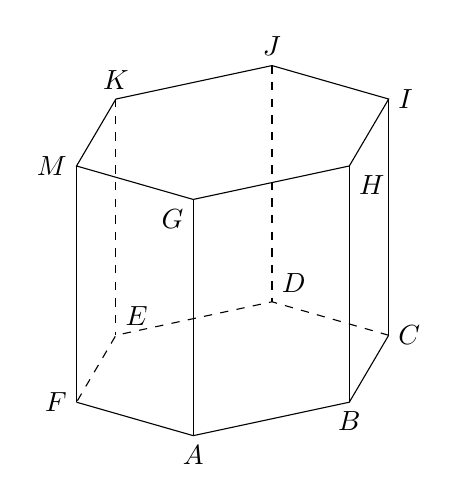
\begin{tikzpicture}[x={(-0.5cm,-0.85cm)},y={(2cm,0cm)},z={(0cm,3cm)}]

\foreach \i/\name/\pozice in {0/A/below, 60/B/below, 120/C/right, 180/D/above right, 240/E/above right, 300/F/left} 
{
\draw ({cos(\i)},{sin(\i)},0) coordinate (\name); 
\draw ({cos(\i)},{sin(\i)},0)  node[\pozice] {$\name$};
}

\foreach \i/\name/\pozice in {0/G/below left, 60/H/below right, 120/I/right, 180/J/above, 240/K/above, 300/M/left} 
{
\draw ({cos(\i)},{sin(\i)},1) coordinate (\name); 
\draw ({cos(\i)},{sin(\i)},1)  node[\pozice] {$\name$};
}

\draw (F)--(A)--(B)--(C);
\draw[dashed] (C)--(D)--(E)--(F);
\draw (M)--(G)--(H)--(I)--(J)--(K)--cycle;
\foreach \i/\j in {A/G, B/H/, I/C, F/M}  { \draw (\i)--(\j);  }
\foreach \i/\j in {K/E, J/D}  { \draw[dashed] (\i)--(\j);  }

\end{tikzpicture}

\newpage


% http://msr.vsb.cz/tiket/1615
% Tecny k elipce (kruznice a afinni transformace)
\begin{tikzpicture}[cm={1,-0.2,0.5,0.6,(0,0)}, scale=2]
  \draw (0,0) circle (1);
  \draw[shorten >=-1cm, shorten <=-1cm] (-1,-1)node[below]{$M$}--(1,-1);
  \draw[shorten >=-1cm, shorten <=-1cm] (-1,-1)--(-1,1);
  \draw[shorten >=-1cm, shorten <=-1cm, red] (0,-1)node[below,black]{$2$}--node[pos=1.3,left]{pol�ra}(-1,0)node[left, black]{$1$};
\end{tikzpicture}



\newpage



% OSY: vodorovne y, svisle z, ven z obrazovky x
 

\begin{tikzpicture}[x={(-0.3cm,-0.3cm)},y={(0.35cm,0cm)},z={(0cm,0.9cm)}]
  \def\cm{\,\mathrm{cm}}
  \coordinate (A) at (3,0,0);
  \coordinate (B) at (3,6,0);
  \coordinate (C) at (0,6,0);
  \coordinate (D) at (0,0,0);
  \coordinate (E) at (3,0,4);
  \coordinate (F) at (3,6,4);
  \coordinate (G) at (0,6,4);
  \coordinate (H) at (0,0,4);
  \def\POPISEK#1#2{\draw ($(#1)!2pt!-90:(#2)$)--($(#1)!2pt!90:(#2)$);}
  \def\Stred #1#2#3{ \coordinate (#1) at ($(#2)!0.5!(#3)$); \POPISEK#1#2}
  \Stred RAB
  \Stred KAE
  \Stred MEF
  \Stred LHG
  \Stred PBF
  \Stred QCG
  \begin{scope}[thick]
    \draw (A)--(B)--(C);
    \draw[dashed] (D)--(C);
    \draw[dashed] (D)--(A); %
    \draw (A)--(E)--(H);
    \draw[dashed] (D)--(H);%
    \draw (E)--(F)--(B); %
    \draw (H)--(G)--(C); %
    \draw (F)--(G); %
  \end{scope}
 
  \foreach \bod/\pozice in {A/below, B/below, C/above right, D/above right, E/below left,
    F/below right, G/above right, H/above right, R/below, K/left, P/right, Q/right, M/above right, L/above}
  {\draw (\bod) node[\pozice]{$\bod$};}
 
 
\end{tikzpicture}

\newpage

\end{document}



%%% Local Variables: 
%%% mode: latex
%%% coding: cp1250
%%% TeX-master: t
%%% End: